\documentclass[11pt]{article}


%\input{meta/packages}
%
\usepackage{cite}
\usepackage[T1]{fontenc}
\usepackage{times}
\usepackage{url}
\usepackage{amsmath}
\usepackage{fancyhdr}
\usepackage{fancyvrb}
\usepackage{fancybox}
\usepackage{color}
\usepackage{colortbl}
\usepackage[table]{xcolor}
%\usepackage{tex-helpers/mathpartir}
\usepackage{amssymb}
\usepackage{xspace}
\usepackage{comment}
\usepackage{graphicx}
\graphicspath{{figures/}}
\usepackage{epsfig}
\usepackage{wrapfig}
\usepackage{multirow}
\usepackage{subfig}

% Added listing for code listings
\usepackage{listings}
\usepackage{relsize}
\usepackage{setspace}
\usepackage{sidecap}
\usepackage{algorithm}
\usepackage{algorithmic}

\textwidth=16.5cm 
\textheight=22.5cm 
\textwidth=16.5cm 
\textheight=55.5pc
\topmargin=-0.5cm 
\headsep=0cm 
\headheight=0cm 
\oddsidemargin=0cm
\evensidemargin=0cm 
\marginparwidth=0cm
\parskip=0cm
\itemsep=0.1pt
\parindent=0.5cm

%Set table separation 
\setlength{\tabcolsep}{1pt}

% Allow figures to take up the entire page
\renewcommand\floatpagefraction{.99}
\renewcommand\topfraction{.99}
\renewcommand\bottomfraction{.90}
\renewcommand\textfraction{.01}   
\setcounter{totalnumber}{50}
\setcounter{topnumber}{50}
\setcounter{bottomnumber}{50}

% formatting for grammars
%\input{tex-helpers/obey}
%\input{tex-helpers/grammar}
%\renewcommand{\nonterm}[1]{\mbox{\textit{#1}}}
\newcommand{\oneormore}[1]{#1\ensuremath{^+}}

\newcommand{\opt}[1]{\textbf{[}#1\textbf{]}}

\newcommand{\mc}[1]{\mbox{\rm \ensuremath{\text{\code{#1}}}}} 
\newcommand{\loc}{\ensuremath{\mathord{\mathit{loc}}}}
\newcommand{\ec}{\ensuremath{\mathop{\mathbb{E}}}}
\newcommand{\hole}{\ensuremath{\mathord{\mathit{-}}}}
\newcommand{\reducesto}{\hookrightarrow}

\newcommand*{\seq}[1]{\ensuremath{\left\langle {#1} \right\rangle}}
\newcommand{\config}{\seq}
\newcommand{\udot}{\mathbin{\sqcup \kern-0.53em \cdot \,}}

% Aux functions
\newcommand{\auxFunc}[1]{\ensuremath{\mathop{\mathit{#1}}}}
\newcommand{\concat}{\auxFunc{concat}}
\newcommand{\reverse}{\auxFunc{reverse}}

% Type checking macros
% change symbol type of : from mathrel 
%\DeclareMathSymbol{:}{\mathbin}{operators}{"3A} 
\newcommand{\OK}{\mbox{OK}}
\newcommand{\OKin}{\mbox{OK in }}
\newcommand{\isType}{\mbox{\textit{isType}}}
\newcommand{\isThunkType}{\mbox{\textit{isThunkType}}}
\newcommand{\isClass}{\mbox{\textit{isClass}}}
\newcommand{\Types}{\mbox{\textit{Types}}}
\newcommand{\Names}{\mbox{\textit{Names}}}
\newcommand{\TypeEnv}{\mbox{\textit{TypeEnv}}}
\newcommand{\VD}{\mbox{\textit{VD}}}
\newcommand{\TypesInOrder}{\mbox{\textit{typesInOrder}}}
\newcommand{\dom}{\mbox{\textit{dom}}}
\newcommand{\rng}{\mbox{\textit{rng}}}
\newcommand{\POWERSET}[1]{\mbox{\textit{PowerSet}}(#1)}
\newcommand{\delete}{\mbox{\textit{delete}}}
\newcommand{\mklist}{\mbox{\textit{mksupers}}}
\newcommand{\uminus}{\mbox{$\cup\!\!\!\!-$}}
\newcommand{\iminus}{\mbox{$\cap\!\!\!\!-$}}
\newcommand{\rname}[1]{$\TirName{(#1)}$} % for inline inferrule names
\newcommand{\STO}{\ensuremath{<:}}  % ``subtype of''
\newcommand{\consistent}{\ensuremath{\approx}}

% Notations 
\newcommand{\produces}{\rightsquigarrow}
\newcommand{\refinedBy}{\sqsubseteq}

% Macros for the Figure Editor Example
\newcommand{\FElement}{\mbox{\texttt{FElement}~}}
\newcommand{\ChangedFE}{\mbox{\texttt{changedFE}~}}
\newcommand{\FEChange}{\mbox{\texttt{FEChange}~}}


% Macros for defining phase transition analysis
\newcommand{\cfg}{\ensuremath{{\cal CFG}}\xspace}
\newcommand{\globTypeMap}{\ensuremath{T}\xspace}

%Redefinition of some math commands widely used outside
%mathmode
\newcommand{\memOf}{\ensuremath{\in}\xspace}

% Help LaTeX not violate the column margins
\tolerance=50000

% settings for listings
\definecolor{lightgray}{gray}{0.97}
\definecolor{darkgray}{gray}{0.5}
\definecolor{OliveGreen}{cmyk}{0.64,0,0.95,0.40}
\definecolor{DarkGreen}{cmyk}{0.58,0,0.66,0.26}
\definecolor{LightRed}{cmyk}{0,0.682,0.728,0}
\definecolor{purple}{cmyk}{0.41,0.73,0,0}

\lstset{
	language=bash, emph={},
	mathescape=false, escapechar=@,
	backgroundcolor=\color{lightgray},
	commentstyle=\color{darkgray},
	keywordstyle=\color{OliveGreen}\bfseries,
	basicstyle=\relsize{-3}\sffamily,
	numberstyle=\scriptsize\sffamily,
	emphstyle=\color{purple},
	emphstyle={[2]\color{LightRed}},
	commentstyle=\color{DarkGreen},
	stringstyle=\color{OliveGreen},
	numbers=left, stepnumber=1,
	numberblanklines=false,
	numberstyle=\tiny,
	numbersep=-3pt,
	frame=none, framexleftmargin=0pt, framexrightmargin=0pt, 
	%xleftmargin=15pt, xrightmargin=4pt,
	columns=flexible, breaklines=true,
	showspaces=false, showstringspaces=false, showtabs=false, tabsize=2,
	morekeywords={input,exists,foreach,ifall,output,of,weight,stop,visit,before,after},
	emph={int,string,bool,time,array,stack,map,visitor,%
true,false,%
top,sum,mean,maximum,minimum,set,collection,%
Project,CodeRepository,Revision,ChangedFile,ASTRoot,Namespace,Declaration,Type,Method,Variable,Statement,Expression,Modifier,%
ExpressionKind,NEW,LITERAL,EQ,NEQ,%
TypeKind,CLASS,ANONYMOUS,%
ModifierKind,OTHER,%
ChangeKind,DELETED,%
StatementKind,IF,%
RepositoryKind,SVN},
	emph={[2]isfixingrevision,getast,iskind,hasfiletype,isliteral,getsnapshot,has_modifier_public,%
format,def,len,match,lowercase,yearof,haskey,remove,strfind,push,pop},
}

% could use \relsize{-2} instead of \scriptsize below
\newcommand{\FIGCODEFONT}{\relsize{-2.5}\ttfamily}

% cross referencing
%\newcommand{\algref}[1]{Algorithm~\ref{#1}}
%\newcommand{\figref}[1]{Figure~\ref{#1}\xspace}
%\newcommand{\tabref}[1]{Table~\ref{#1}\xspace}
%\newcommand{\fignref}[1]{Figure~\ref{#1}\xspace}
%\newcommand{\secref}[1]{Section~\ref{#1}\xspace}
%\newcommand{\secnref}[1]{Section~\ref{#1}\xspace}

%\newcommand{\etal}{~\textit{et al.}\@\xspace}
\newcommand{\kind}{\textit{kind}\xspace}
\newcommand{\KIND}{\textit{KIND}\xspace}

\newcommand{\lang}{\textit{Boa}\@\xspace}

% Theorems environments...
%{theorems}
\newtheorem{theorem}{Theorem}[section]
\newtheorem{axiom}[theorem]{Axiom}
\newtheorem{corollary}[theorem]{Corollary}
\newtheorem{definition}[theorem]{Definition}
\newtheorem{example}[theorem]{Example}
\newtheorem{fact}[theorem]{Fact}
\newtheorem{lemma}[theorem]{Lemma}
\newtheorem{proposition}[theorem]{Proposition}
\newtheorem{remark}[theorem]{Remark}
\newtheorem{conjecture}[theorem]{Conjecture}
% Some helpful notation
\newcommand{\PROOF}{{\em Proof:\/}~~}
\newcommand{\PROOFSKETCH}{{\em Proof Sketch:\/}~~}
\newcommand{\QED}{\rule{0.4em}{0.65em}}

\definecolor{light-gray}{gray}{0.9}
\definecolor{very-light-gray}{gray}{0.95}

% Change section headings to look nicer
\makeatletter
\renewcommand\thesection{{\large\Alph{section}.}}
\renewcommand\section{\@startsection {section}{1}{\z@}%
                                   {-3.5ex \@plus -1ex \@minus -.2ex}%
                                   {2.3ex \@plus.2ex}%
                                   {\large\scshape\bf}}
\makeatother

\renewcommand\thesubsection{{\normalsize\Alph{section}.}{\normalsize\arabic{subsection}}}

\makeatletter
\renewcommand\subsection{\@startsection {subsection}{1}{\z@}%
                                   {-3.5ex \@plus -1ex \@minus -.2ex}%
                                   {2.3ex \@plus.2ex}%
                                   {\normalsize\scshape\bf}}
\makeatother

\renewcommand\thesubsubsection{{\normalsize\Alph{section}.}{\normalsize\arabic{subsection}.}{\normalsize\arabic{subsubsection}}}

\makeatletter
\renewcommand\subsubsection{\@startsection {subsubsection}{1}{\z@}%
                                   {-3.5ex \@plus -1ex \@minus -.2ex}%
                                   {2.3ex \@plus.2ex}%
                                   {\normalsize\scshape\bf}}
\makeatother

\newcommand\para[1]{\vspace{-1em}\paragraph{#1\ }}

% Different font in captions
\newcommand{\captionfonts}{\footnotesize}

% formatting of initial section quotations
\newcommand{\QUOTATION}[1]{\begin{flushright}\begin{footnotesize}\emph{#1}\end{footnotesize}\end{flushright}}
 
\makeatletter  % Allow the use of @ in command names
\long\def\@makecaption#1#2{%
  \vskip\abovecaptionskip
  \sbox\@tempboxa{{\captionfonts #1: #2}}%
  \ifdim \wd\@tempboxa >\hsize
    {\captionfonts #1: #2\par}
  \else
    \hbox to\hsize{\hfil\box\@tempboxa\hfil}%
  \fi
  \vskip\belowcaptionskip}
\makeatother   % Cancel the effect of \makeatletter

%\usepackage[ps2pdf,bookmarks=true]{hyperref}

\definecolor{light-gray}{gray}{0.9}
\definecolor{dark-gray}{gray}{0.7}

\newcommand\doctitle[1]{\newpage \setcounter{page}{1}\thispagestyle{fancyplain} \headheight=14pt%
                        \fancyhead[C]{\large{\bf #1}}\xspace\vspace{0.5em}}


                                                                        


\usepackage{graphicx,times}
\usepackage{wrapfig}
\usepackage{amsmath,epsfig}
\usepackage{setspace,array}
\usepackage{cite}
\usepackage{listings}
\usepackage{booktabs}
%\usepackage{bibentry}
\lstset{basicstyle=\scriptsize\sffamily,language={},frame=single,breaklines=true,columns=fullflexible,mathescape=true,escapechar=@}

\usepackage{tikz}
\newcommand*\circled[1]{\tikz[baseline=(char.base)]{
		\node[shape=circle,draw,inner sep=0.45pt] (char) {#1};}}


\usepackage{xspace}
\usepackage{enumitem}

\usepackage{sectsty}
\sectionfont{\large}
\subsectionfont{\normalsize}
\subsubsectionfont{\normalsize}

\usepackage[compact]{titlesec}
\usepackage[skins]{tcolorbox}

\renewcommand{\theequation}{\thesection.\arabic{equation}}
\renewcommand{\baselinestretch}{1.0}

\newcommand*\rotdia{\multicolumn{1}{R{45}{1em}}}% no optional argument here, please!
\newcommand*\rot{\rotatebox{90}}
\usepackage{multicol,multirow}

\newtheorem{Definition}{Definition}
\newtheorem{Claim}{Claim}
\newtheorem{Lemma}{Lemma}
\newtheorem{Theorem}{Theorem}
\newtheorem{Property}{Property}
\newtheorem{Problem}{Problem}


\newcommand\aName[1]{{\small\textsc{#1}}\xspace}

% cross referencing
\newcommand{\figref}[1]{Figure~\ref{#1}}
\newcommand{\secref}[1]{Section~\ref{#1}}
\newcommand{\tabref}[1]{Table~\ref{#1}}
\newcommand{\defref}[1]{Definition~\ref{#1}}

%\newcommand\aName[1]{{\small\textnormal{\textsc{#1}}}\xspace}

%\newcommand\MUBench[0]{\aName{MuBench}}
\newcommand\MUDetect[0]{\aName{MuDetect}}



\newcommand\MUBench[0]{\aName{MuBench}}
\newcommand\MUPipe[0]{\aName{MuPipe}}
\newcommand\MUC[0]{\aName{MuC}}
\newcommand\AUG[0]{\aName{AUG}}

\newcommand{\etal}{{\em et al.}}

\newcommand\GROUM[0]{\aName{GROUM}}
\newcommand\eGROUM[0]{\aName{AUG}}
\newcommand\miner[0]{\aName{AUGMiner}}

\newcommand\Colibri[0]{\aName{Colibri/ML}}
\newcommand\DroidAssist[0]{\aName{DroidAssist}}
\newcommand\GraPacc[0]{\aName{GraPacc}}
\newcommand\GROUMiner[0]{\aName{GROUMiner}}
\newcommand\Jadet[0]{\aName{Jadet}}
\newcommand\PRMiner[0]{\aName{PR-Miner}}
\newcommand\CARMiner[0]{\aName{CAR-Miner}}
\newcommand\Alattin[0]{\aName{Alattin}}
\newcommand\Tikanga[0]{\aName{Tikanga}}
\newcommand\DMMC[0]{\aName{DMMC}}
\newcommand\RGJ[0]{\aName{RGJ07}}
\newcommand\Chronicler[0]{\aName{Chronicler}}
\newcommand\Acharya[0]{\aName{AX09}}

\newcommand{\checkNum}[1]{#1}

\newcommand{\revise} {\bf}

\newcommand{\code}[1]{{\scriptsize\texttt{#1}}}
\newcommand{\op}{\tau}
\newcommand{\refac}{\rho}
\newcommand{\edit}{\sigma}
\newcommand{\T}{\theta}
\newcommand{\comp}{;}
\newcommand{\pre}{\prec_P}
\newcommand{\meth}{KSISA}

\newcommand{\MyParagraph}[1]{\textbf{#1}{ }}
\newcommand{\fixme} [1] {\textcolor{red}{{\it FIXME}: #1}}

\usepackage{vmargin}
\setpapersize{USletter}
\setmarginsrb{1.0in}{1in}{1.0in}{1in}%
           {0pt}{0mm}{0pt}{10mm}
\newcommand{\remove}[1]{}



\usepackage{tweaklist}
\renewcommand{\enumhook}{\setlength{\topsep}{0pt}%
  \setlength{\itemsep}{0pt}}
\renewcommand{\itemhook}{\setlength{\topsep}{0pt}%
  \setlength{\itemsep}{0pt}}
\renewcommand{\descripthook}{\setlength{\topsep}{0pt}%
  \setlength{\itemsep}{0pt}}



%\newcommand\Tone{Thrust 1 (T1). Ongoing Evaluation of Existing Code Representation Learning in Bug Detect-Fix Processes}
\newcommand\Tone{Thrust 1 (T1). Design Framework and Environment for Code Representation Learning (CRL): Representations, Models, and Methodologies}

\newcommand\Ttwo{Thrust 2 (T2). Quality Evaluation Framework for Code Representation Learning}

\newcommand\Tthree{Thrust 3 (T3). Applications of CRL Framework in Bug Detection, Testing, Fault Localization, and Auto Program Repair}

%Enhancing Techniques in the Bug Fixing Process with Deep Learning}

% all tool names used in this proposal

%\newcommand\tool{NeuralPPA}

\newcommand{\tool}{\textsc{NeuralPA}\xspace}
\newcommand{\deeppda}{\textsc{DeepPDA}\xspace}

\newcommand\deepbugs{\textbf{DeepBugs}~\cite{Pradel-2018}}
\newcommand\bugram{\textbf{Bugram}~\cite{Wang-2016}}
\newcommand\narminer{\textbf{NAR-miner}~\cite{Bian-2018}}
\newcommand\findbugs{\textbf{FindBugs}~\cite{ayewah-2007}}
\newcommand\deepsim{\textbf{DeepSim}\cite{Zhao-2018}}
\newcommand\codetovec{\textbf{code2vec}\cite{Alon-2018}}
\newcommand\codevectors{\textbf{CodeVectors}\cite{Henkel-2018}}
\newcommand\dlsim{\textbf{DL-Sim}~\cite{Tufano-2018}}
\newcommand\treelstm{\textbf{Tree~LSTM}~\cite{Tai-2015}}

\newcommand\cnn{CNN~\cite{kim2014convolutional}}



% auto-fix
\newcommand\CODIT{\textbf{CODIT}~\cite{chakrabortycodit}}
\newcommand\Ratchet{\textbf{Ratchet}~\cite{hata2018learning}}
\newcommand\Tufano{\textbf{Tufano}~\cite{tufano2019learning}}
\newcommand\CoCo{\textbf{CoCoNut}~\cite{lutellier2020coconut}}

% FL
\newcommand\MLP{\textbf{MLP}~\cite{bourlard1988auto}}
\begin{document}

\begin{center}
%{\large \bf Collaborative Research: SHF: Small: Innovations in Deep Learning to Enhance Program Analysis and Representations to Improve Bug Fixing Process}

%{\large \bf Collaborative Research: SHF: Small: Connecting Deep Learning and Program Analysis to Improve Bug Detecting and Fixing Processes through Code Representation Learning}

{\large \bf SaTC: Small: Neural Program Analysis Infrastructure to Support\\ Early Vulnerability Detection}
\end{center}
\vspace{-.1in}
\hrule

%%
\usepackage{cite}
\usepackage[T1]{fontenc}
\usepackage{times}
\usepackage{url}
\usepackage{amsmath}
\usepackage{fancyhdr}
\usepackage{fancyvrb}
\usepackage{fancybox}
\usepackage{color}
\usepackage{colortbl}
\usepackage[table]{xcolor}
%\usepackage{tex-helpers/mathpartir}
\usepackage{amssymb}
\usepackage{xspace}
\usepackage{comment}
\usepackage{graphicx}
\graphicspath{{figures/}}
\usepackage{epsfig}
\usepackage{wrapfig}
\usepackage{multirow}
\usepackage{subfig}

% Added listing for code listings
\usepackage{listings}
\usepackage{relsize}
\usepackage{setspace}
\usepackage{sidecap}
\usepackage{algorithm}
\usepackage{algorithmic}

\textwidth=16.5cm 
\textheight=22.5cm 
\textwidth=16.5cm 
\textheight=55.5pc
\topmargin=-0.5cm 
\headsep=0cm 
\headheight=0cm 
\oddsidemargin=0cm
\evensidemargin=0cm 
\marginparwidth=0cm
\parskip=0cm
\itemsep=0.1pt
\parindent=0.5cm

%Set table separation 
\setlength{\tabcolsep}{1pt}

% Allow figures to take up the entire page
\renewcommand\floatpagefraction{.99}
\renewcommand\topfraction{.99}
\renewcommand\bottomfraction{.90}
\renewcommand\textfraction{.01}   
\setcounter{totalnumber}{50}
\setcounter{topnumber}{50}
\setcounter{bottomnumber}{50}

% formatting for grammars
%\input{tex-helpers/obey}
%\input{tex-helpers/grammar}
%\renewcommand{\nonterm}[1]{\mbox{\textit{#1}}}
\newcommand{\oneormore}[1]{#1\ensuremath{^+}}

\newcommand{\opt}[1]{\textbf{[}#1\textbf{]}}

\newcommand{\mc}[1]{\mbox{\rm \ensuremath{\text{\code{#1}}}}} 
\newcommand{\loc}{\ensuremath{\mathord{\mathit{loc}}}}
\newcommand{\ec}{\ensuremath{\mathop{\mathbb{E}}}}
\newcommand{\hole}{\ensuremath{\mathord{\mathit{-}}}}
\newcommand{\reducesto}{\hookrightarrow}

\newcommand*{\seq}[1]{\ensuremath{\left\langle {#1} \right\rangle}}
\newcommand{\config}{\seq}
\newcommand{\udot}{\mathbin{\sqcup \kern-0.53em \cdot \,}}

% Aux functions
\newcommand{\auxFunc}[1]{\ensuremath{\mathop{\mathit{#1}}}}
\newcommand{\concat}{\auxFunc{concat}}
\newcommand{\reverse}{\auxFunc{reverse}}

% Type checking macros
% change symbol type of : from mathrel 
%\DeclareMathSymbol{:}{\mathbin}{operators}{"3A} 
\newcommand{\OK}{\mbox{OK}}
\newcommand{\OKin}{\mbox{OK in }}
\newcommand{\isType}{\mbox{\textit{isType}}}
\newcommand{\isThunkType}{\mbox{\textit{isThunkType}}}
\newcommand{\isClass}{\mbox{\textit{isClass}}}
\newcommand{\Types}{\mbox{\textit{Types}}}
\newcommand{\Names}{\mbox{\textit{Names}}}
\newcommand{\TypeEnv}{\mbox{\textit{TypeEnv}}}
\newcommand{\VD}{\mbox{\textit{VD}}}
\newcommand{\TypesInOrder}{\mbox{\textit{typesInOrder}}}
\newcommand{\dom}{\mbox{\textit{dom}}}
\newcommand{\rng}{\mbox{\textit{rng}}}
\newcommand{\POWERSET}[1]{\mbox{\textit{PowerSet}}(#1)}
\newcommand{\delete}{\mbox{\textit{delete}}}
\newcommand{\mklist}{\mbox{\textit{mksupers}}}
\newcommand{\uminus}{\mbox{$\cup\!\!\!\!-$}}
\newcommand{\iminus}{\mbox{$\cap\!\!\!\!-$}}
\newcommand{\rname}[1]{$\TirName{(#1)}$} % for inline inferrule names
\newcommand{\STO}{\ensuremath{<:}}  % ``subtype of''
\newcommand{\consistent}{\ensuremath{\approx}}

% Notations 
\newcommand{\produces}{\rightsquigarrow}
\newcommand{\refinedBy}{\sqsubseteq}

% Macros for the Figure Editor Example
\newcommand{\FElement}{\mbox{\texttt{FElement}~}}
\newcommand{\ChangedFE}{\mbox{\texttt{changedFE}~}}
\newcommand{\FEChange}{\mbox{\texttt{FEChange}~}}


% Macros for defining phase transition analysis
\newcommand{\cfg}{\ensuremath{{\cal CFG}}\xspace}
\newcommand{\globTypeMap}{\ensuremath{T}\xspace}

%Redefinition of some math commands widely used outside
%mathmode
\newcommand{\memOf}{\ensuremath{\in}\xspace}

% Help LaTeX not violate the column margins
\tolerance=50000

% settings for listings
\definecolor{lightgray}{gray}{0.97}
\definecolor{darkgray}{gray}{0.5}
\definecolor{OliveGreen}{cmyk}{0.64,0,0.95,0.40}
\definecolor{DarkGreen}{cmyk}{0.58,0,0.66,0.26}
\definecolor{LightRed}{cmyk}{0,0.682,0.728,0}
\definecolor{purple}{cmyk}{0.41,0.73,0,0}

\lstset{
	language=bash, emph={},
	mathescape=false, escapechar=@,
	backgroundcolor=\color{lightgray},
	commentstyle=\color{darkgray},
	keywordstyle=\color{OliveGreen}\bfseries,
	basicstyle=\relsize{-3}\sffamily,
	numberstyle=\scriptsize\sffamily,
	emphstyle=\color{purple},
	emphstyle={[2]\color{LightRed}},
	commentstyle=\color{DarkGreen},
	stringstyle=\color{OliveGreen},
	numbers=left, stepnumber=1,
	numberblanklines=false,
	numberstyle=\tiny,
	numbersep=-3pt,
	frame=none, framexleftmargin=0pt, framexrightmargin=0pt, 
	%xleftmargin=15pt, xrightmargin=4pt,
	columns=flexible, breaklines=true,
	showspaces=false, showstringspaces=false, showtabs=false, tabsize=2,
	morekeywords={input,exists,foreach,ifall,output,of,weight,stop,visit,before,after},
	emph={int,string,bool,time,array,stack,map,visitor,%
true,false,%
top,sum,mean,maximum,minimum,set,collection,%
Project,CodeRepository,Revision,ChangedFile,ASTRoot,Namespace,Declaration,Type,Method,Variable,Statement,Expression,Modifier,%
ExpressionKind,NEW,LITERAL,EQ,NEQ,%
TypeKind,CLASS,ANONYMOUS,%
ModifierKind,OTHER,%
ChangeKind,DELETED,%
StatementKind,IF,%
RepositoryKind,SVN},
	emph={[2]isfixingrevision,getast,iskind,hasfiletype,isliteral,getsnapshot,has_modifier_public,%
format,def,len,match,lowercase,yearof,haskey,remove,strfind,push,pop},
}

% could use \relsize{-2} instead of \scriptsize below
\newcommand{\FIGCODEFONT}{\relsize{-2.5}\ttfamily}

% cross referencing
%\newcommand{\algref}[1]{Algorithm~\ref{#1}}
%\newcommand{\figref}[1]{Figure~\ref{#1}\xspace}
%\newcommand{\tabref}[1]{Table~\ref{#1}\xspace}
%\newcommand{\fignref}[1]{Figure~\ref{#1}\xspace}
%\newcommand{\secref}[1]{Section~\ref{#1}\xspace}
%\newcommand{\secnref}[1]{Section~\ref{#1}\xspace}

%\newcommand{\etal}{~\textit{et al.}\@\xspace}
\newcommand{\kind}{\textit{kind}\xspace}
\newcommand{\KIND}{\textit{KIND}\xspace}

\newcommand{\lang}{\textit{Boa}\@\xspace}

% Theorems environments...
%{theorems}
\newtheorem{theorem}{Theorem}[section]
\newtheorem{axiom}[theorem]{Axiom}
\newtheorem{corollary}[theorem]{Corollary}
\newtheorem{definition}[theorem]{Definition}
\newtheorem{example}[theorem]{Example}
\newtheorem{fact}[theorem]{Fact}
\newtheorem{lemma}[theorem]{Lemma}
\newtheorem{proposition}[theorem]{Proposition}
\newtheorem{remark}[theorem]{Remark}
\newtheorem{conjecture}[theorem]{Conjecture}
% Some helpful notation
\newcommand{\PROOF}{{\em Proof:\/}~~}
\newcommand{\PROOFSKETCH}{{\em Proof Sketch:\/}~~}
\newcommand{\QED}{\rule{0.4em}{0.65em}}

\definecolor{light-gray}{gray}{0.9}
\definecolor{very-light-gray}{gray}{0.95}

% Change section headings to look nicer
\makeatletter
\renewcommand\thesection{{\large\Alph{section}.}}
\renewcommand\section{\@startsection {section}{1}{\z@}%
                                   {-3.5ex \@plus -1ex \@minus -.2ex}%
                                   {2.3ex \@plus.2ex}%
                                   {\large\scshape\bf}}
\makeatother

\renewcommand\thesubsection{{\normalsize\Alph{section}.}{\normalsize\arabic{subsection}}}

\makeatletter
\renewcommand\subsection{\@startsection {subsection}{1}{\z@}%
                                   {-3.5ex \@plus -1ex \@minus -.2ex}%
                                   {2.3ex \@plus.2ex}%
                                   {\normalsize\scshape\bf}}
\makeatother

\renewcommand\thesubsubsection{{\normalsize\Alph{section}.}{\normalsize\arabic{subsection}.}{\normalsize\arabic{subsubsection}}}

\makeatletter
\renewcommand\subsubsection{\@startsection {subsubsection}{1}{\z@}%
                                   {-3.5ex \@plus -1ex \@minus -.2ex}%
                                   {2.3ex \@plus.2ex}%
                                   {\normalsize\scshape\bf}}
\makeatother

\newcommand\para[1]{\vspace{-1em}\paragraph{#1\ }}

% Different font in captions
\newcommand{\captionfonts}{\footnotesize}

% formatting of initial section quotations
\newcommand{\QUOTATION}[1]{\begin{flushright}\begin{footnotesize}\emph{#1}\end{footnotesize}\end{flushright}}
 
\makeatletter  % Allow the use of @ in command names
\long\def\@makecaption#1#2{%
  \vskip\abovecaptionskip
  \sbox\@tempboxa{{\captionfonts #1: #2}}%
  \ifdim \wd\@tempboxa >\hsize
    {\captionfonts #1: #2\par}
  \else
    \hbox to\hsize{\hfil\box\@tempboxa\hfil}%
  \fi
  \vskip\belowcaptionskip}
\makeatother   % Cancel the effect of \makeatletter

%\usepackage[ps2pdf,bookmarks=true]{hyperref}

\definecolor{light-gray}{gray}{0.9}
\definecolor{dark-gray}{gray}{0.7}

\newcommand\doctitle[1]{\newpage \setcounter{page}{1}\thispagestyle{fancyplain} \headheight=14pt%
                        \fancyhead[C]{\large{\bf #1}}\xspace\vspace{0.5em}}


                                                                        


%\input{outline}

\section{Introduction}



%%\subsection{Problem Description}


Developers often use online question and answering (Q\&A) forums,
e.g., StackOverflow (S/O), to learn how to use software libraries and
frameworks. Sometimes, the answer to a question comes as a
fragment/chunk of code, which later makes it to the production
applications, stemming from the copy-and-paste software reuse
practice. Unfortunately, if the copied code fragments are vulnerable,
i.e., possess defects that can potentially be exploited, it will lead
to the applications being prone to attacks. Verdi {\em et
  al.}~\cite{verdi-tse22} reviewed more than 72K C++ code snippets
that migrated from 1,325 S/O answers. Of these, they reported a total
of 99 vulnerable code snippets of 31 different types that made their
way to 2,589 GitHub repositories. Thus, it is crucial to detect early
the vulnerabilities in the code snippets from online forums.
%Running a vulnerability detection tool on the source code after the
%integration of a S/O code snippet into the current codebase would
%waste developers' effort for such integration.

Security researchers have proposed several automated approaches for
vulnerability detection (VD) using program
analysis~\cite{FlawFinder,RATS,viega2000its4,Checkmarx,HPFortify,Coverity,BufferOverFlow,SQLInj,Cross-siteScripting,AuthBypassSpoofing},
as well as machine learning (ML) including deep learning
(DL)~\cite{fse21,chakraborty2020deep,zhou2019devign,li2018sysevr,li2018vuldeepecker}
techniques. However, these approaches warrant the code to exist as
complete program units, often making use of program representations
such~as abstract syntax tree (AST), Program Dependence Graph
(PDG)~\cite{fse21,li2018vuldeepecker}, Control Flow Graph
(CFG)~\cite{zhou2019devign}, Data Flow Graph
(DFG)~\cite{zhou2019devign}, Code Property Graph
(CPG)~\cite{chakraborty2020deep}, etc. At a minimum, they operate at
the method-level granularity, making it impossible to utilize them for
directly detecting vulnerabilities in code snippets. A possible
alternative would be to plug the code snippet into the method, resolve
any ambiguities, and test it with a VD tool. However, such a strategy
is limited. First, if found vulnerable, the efforts of integrating the
code snippet into the existing method would be lost. Second, due to
the black-box
%(inexplicable?)
nature of DL models, we would not know the origin of the
vulnerability, i.e., whether it arises due to the flawed code snippet
or the existing part of the code.

%other statements in the method.

%Besides, even a commit-level VD model requires the code before/after changes to be syntactically valid to extract those features.

Importantly, analyzing code snippets is not straightforward as they
are often incomplete, un-parseable, contain declaration/reference
ambiguity, and are interspersed between user comments. Currently,
there exist tools such as PPA~\cite{ppa08},~which parse an incomplete
code fragment to build the AST and~ex\-tract data types in a
best-effort manner, while StaType \cite{icse18} resolves the libraries
and recovers only the fully-qualified names for references. However,
the basic infrastructure for partial program analysis on incomplete
code snippets is not yet possible. The infrastructure includes the
fundamental supports/services such as lexical, syntactic, and semantic
analysis so that the static and dynamic analysis techniques could be
built upon. Let us call such an infrastructure, {\em partial program
analysis infrastructure}.

In addition to vulnerability detection, such partial program analysis
infrastructure is also beneficial to the other software engineering
(SE) tasks that can tolerate a low level of errors and imprecision in
building the program representations. For example, consider code
completion~\cite{codefill-icse22,facebook-icse21}, in which a model
provides suggestions to complete partial code. Existing ML/DL-based
code completion models are just based on the code sequences or utilize
the syntactic structure in ASTs, but none leverage the program
dependencies due to the nature of partial code. Next, consider the
task of analyzing the code fragments in a bug report to connect it to
the relevant source files for bug localization
purposes~\cite{euler-fse19,icpc17}. Here too, a need for partial
program analysis, especially for partial program dependence analysis,
can be observed.









%\section{Introduction}
Integrating the utilization of program analysis (PA) tools early in the development process of modern, large-scale software systems is crucial in determining the weaknesses/vulnerabilities in the code. Consider, for instance, a scenario in which a developer wants to use an online question and answering (Q\&A) forum, e.g., StackOverflow (S/O), to learn how to use software libraries or frameworks. Typically, the answer to a posed question comes as a fragment/chunk of code, which later makes it to the production application, stemming from the copy-and-paste software reuse practice. Unfortunately, if the copied code fragment is vulnerable, i.e., possesses defects that one can potentially exploit, it will result in the application being prone to attacks. Verdi {\em et al.}~\cite{verdi-tse22} reviewed more than 72K C++ code snippets that migrated from 1,325 S/O answers, reporting a total of 99 vulnerable code snippets of 31 different types that made their way to 2,589 GitHub repositories.

Security researchers have proposed several automated approaches for vulnerability detection (VD) in software systems using program analysis (PA)~\cite{FlawFinder,RATS,viega2000its4,Checkmarx,HPFortify,Coverity}, as well as machine and deep learning (ML \& DL) \cite{fse21,chakraborty2020deep,zhou2019devign,li2018sysevr,li2018vuldeepecker} techniques. These approaches typically leverage program representations such as abstract syntax tree (AST), program dependence graph (PDG)~\cite{fse21,li2018vuldeepecker}, control-flow graph (CFG)~\cite{zhou2019devign}, data-flow graph (DFG)~\cite{zhou2019devign}, code property graph (CPG)~\cite{chakraborty2020deep}, etc., to model the vulnerable features. 
%However, extending such analyses to code snippets is not straightforward as they are often incomplete, unparseable, contain declaration/reference ambiguity, and may be interspersed between user comments. Currently, there exist tools such as PPA~\cite{ppa08}, which parse an incomplete code fragment to build the AST and extract data types in a best-effort manner, while StaType \cite{icse18} resolves the libraries and recovers only the fully-qualified names for references. However, the basic infrastructure for partial program analysis, i.e., for analyzing incomplete code is not yet available. 
%Such an infrastructure must include fundamental supports/services at the structural, semantic, and execution levels, thus enabling the static and dynamic analysis techniques to be built upon. 
%Let us refer to this as \textit{partial program analysis infrastructure}.
However, the PA tools employed to derive these program representations warrant the code to exist as complete program units, at the very least, at the method-level granularity. As a result, it is impossible to utilize such VD tools to find vulnerabilities in code snippets. A possible alternative would be to plug the code snippet into the method, resolve any ambiguities, and test it with a VD tool. However, such a strategy is limited. First, if a vulnerability is found, the efforts of integrating the code snippet into the existing method would be lost. Second, due to the black-box nature of DL models, we would not know the origin of the vulnerability, i.e., whether it arises due to the flawed code snippet or the existing part of the code.

Besides, analyzing code snippets is not straightforward as they are often incomplete, un-parseable, contain declaration/reference ambiguity, and may be interspersed between user comments. Currently, there exist tools such as PPA~\cite{ppa08},~which parse an incomplete code fragment to build the AST and extract data types in a best-effort manner, while StatType \cite{icse18} resolves the libraries and recovers only the fully-qualified names for references. However, the basic infrastructure for partial program analysis, i.e., for analyzing incomplete code is not yet available. Such an infrastructure must include fundamental supports/services at the structural and semantic levels, thus enabling the program analysis techniques to be built upon. Let us refer to this as \textit{partial program analysis infrastructure}.


In addition to vulnerability detection, such an 
%partial program analysis infrastructure 
infrastructure
is also beneficial to other software engineering (SE) tasks that can tolerate a low level of errors and imprecision in building program representations. For example, consider code completion~\cite{codefill-icse22,facebook-icse21}, in which a model provides suggestions to complete partial code. Existing state-of-the-art ML/DL-based code completion models are just based on the code sequences or utilize the syntactic structure in ASTs, but none leverage the program dependencies due to the nature of partial code. Next, consider the task of analyzing the code fragments in a bug report to connect it to the relevant source files for bug localization purposes~\cite{euler-fse19,icpc17}. Here too, a need for partial program analysis, specifically partial program dependence analysis, can be observed.

The other facets of program analysis tools that need to be considered are their soundness and completeness. For example, static analysis tools are designed to detect errors that are valid for all possible executions, which often come at the cost of multiple approximations. As a result, such tools tend to overestimate, resulting in false positives. Next, consider the task of symbolic execution, which is limited by the path explosion problem that hinders its applicability to large-scale software systems. The effectiveness of such a symbolic execution engine can be improved by enhancing the symbolic constraints of the variables, and by guiding it to explore the right subset of symbolic states. 

%While the state-of-the-art research and practice has been well-established for the analysis of the entire programs, very little research and knowledge has been achieved for partial program analysis.

To this effect, we set out to investigate {\tool}, a {\em \underline{Neural} Network-Based \underline{P}rogram \underline{A}nalysis} infrastructure. We aim to establish {\em a scientific foundation, novel methodologies, frameworks, models, and algorithmic solutions for neural program analysis}. We address two major issues in Program Analysis:

(1) {\bf Enabling analysis of incomplete code fragments}, i.e.,
partial program analysis;

(2) {\bf Empowering existing PA tools by making them more sound and
  complete} (Figure~\ref{fig:arch}). {\tool} will allow the
construction of efficient program analysis techniques for (partial)
code on which downstream software engineering applications can be
built.


\subsection{Research Objectives and Anticipated Results}

\begin{figure}[t]
    \centering
    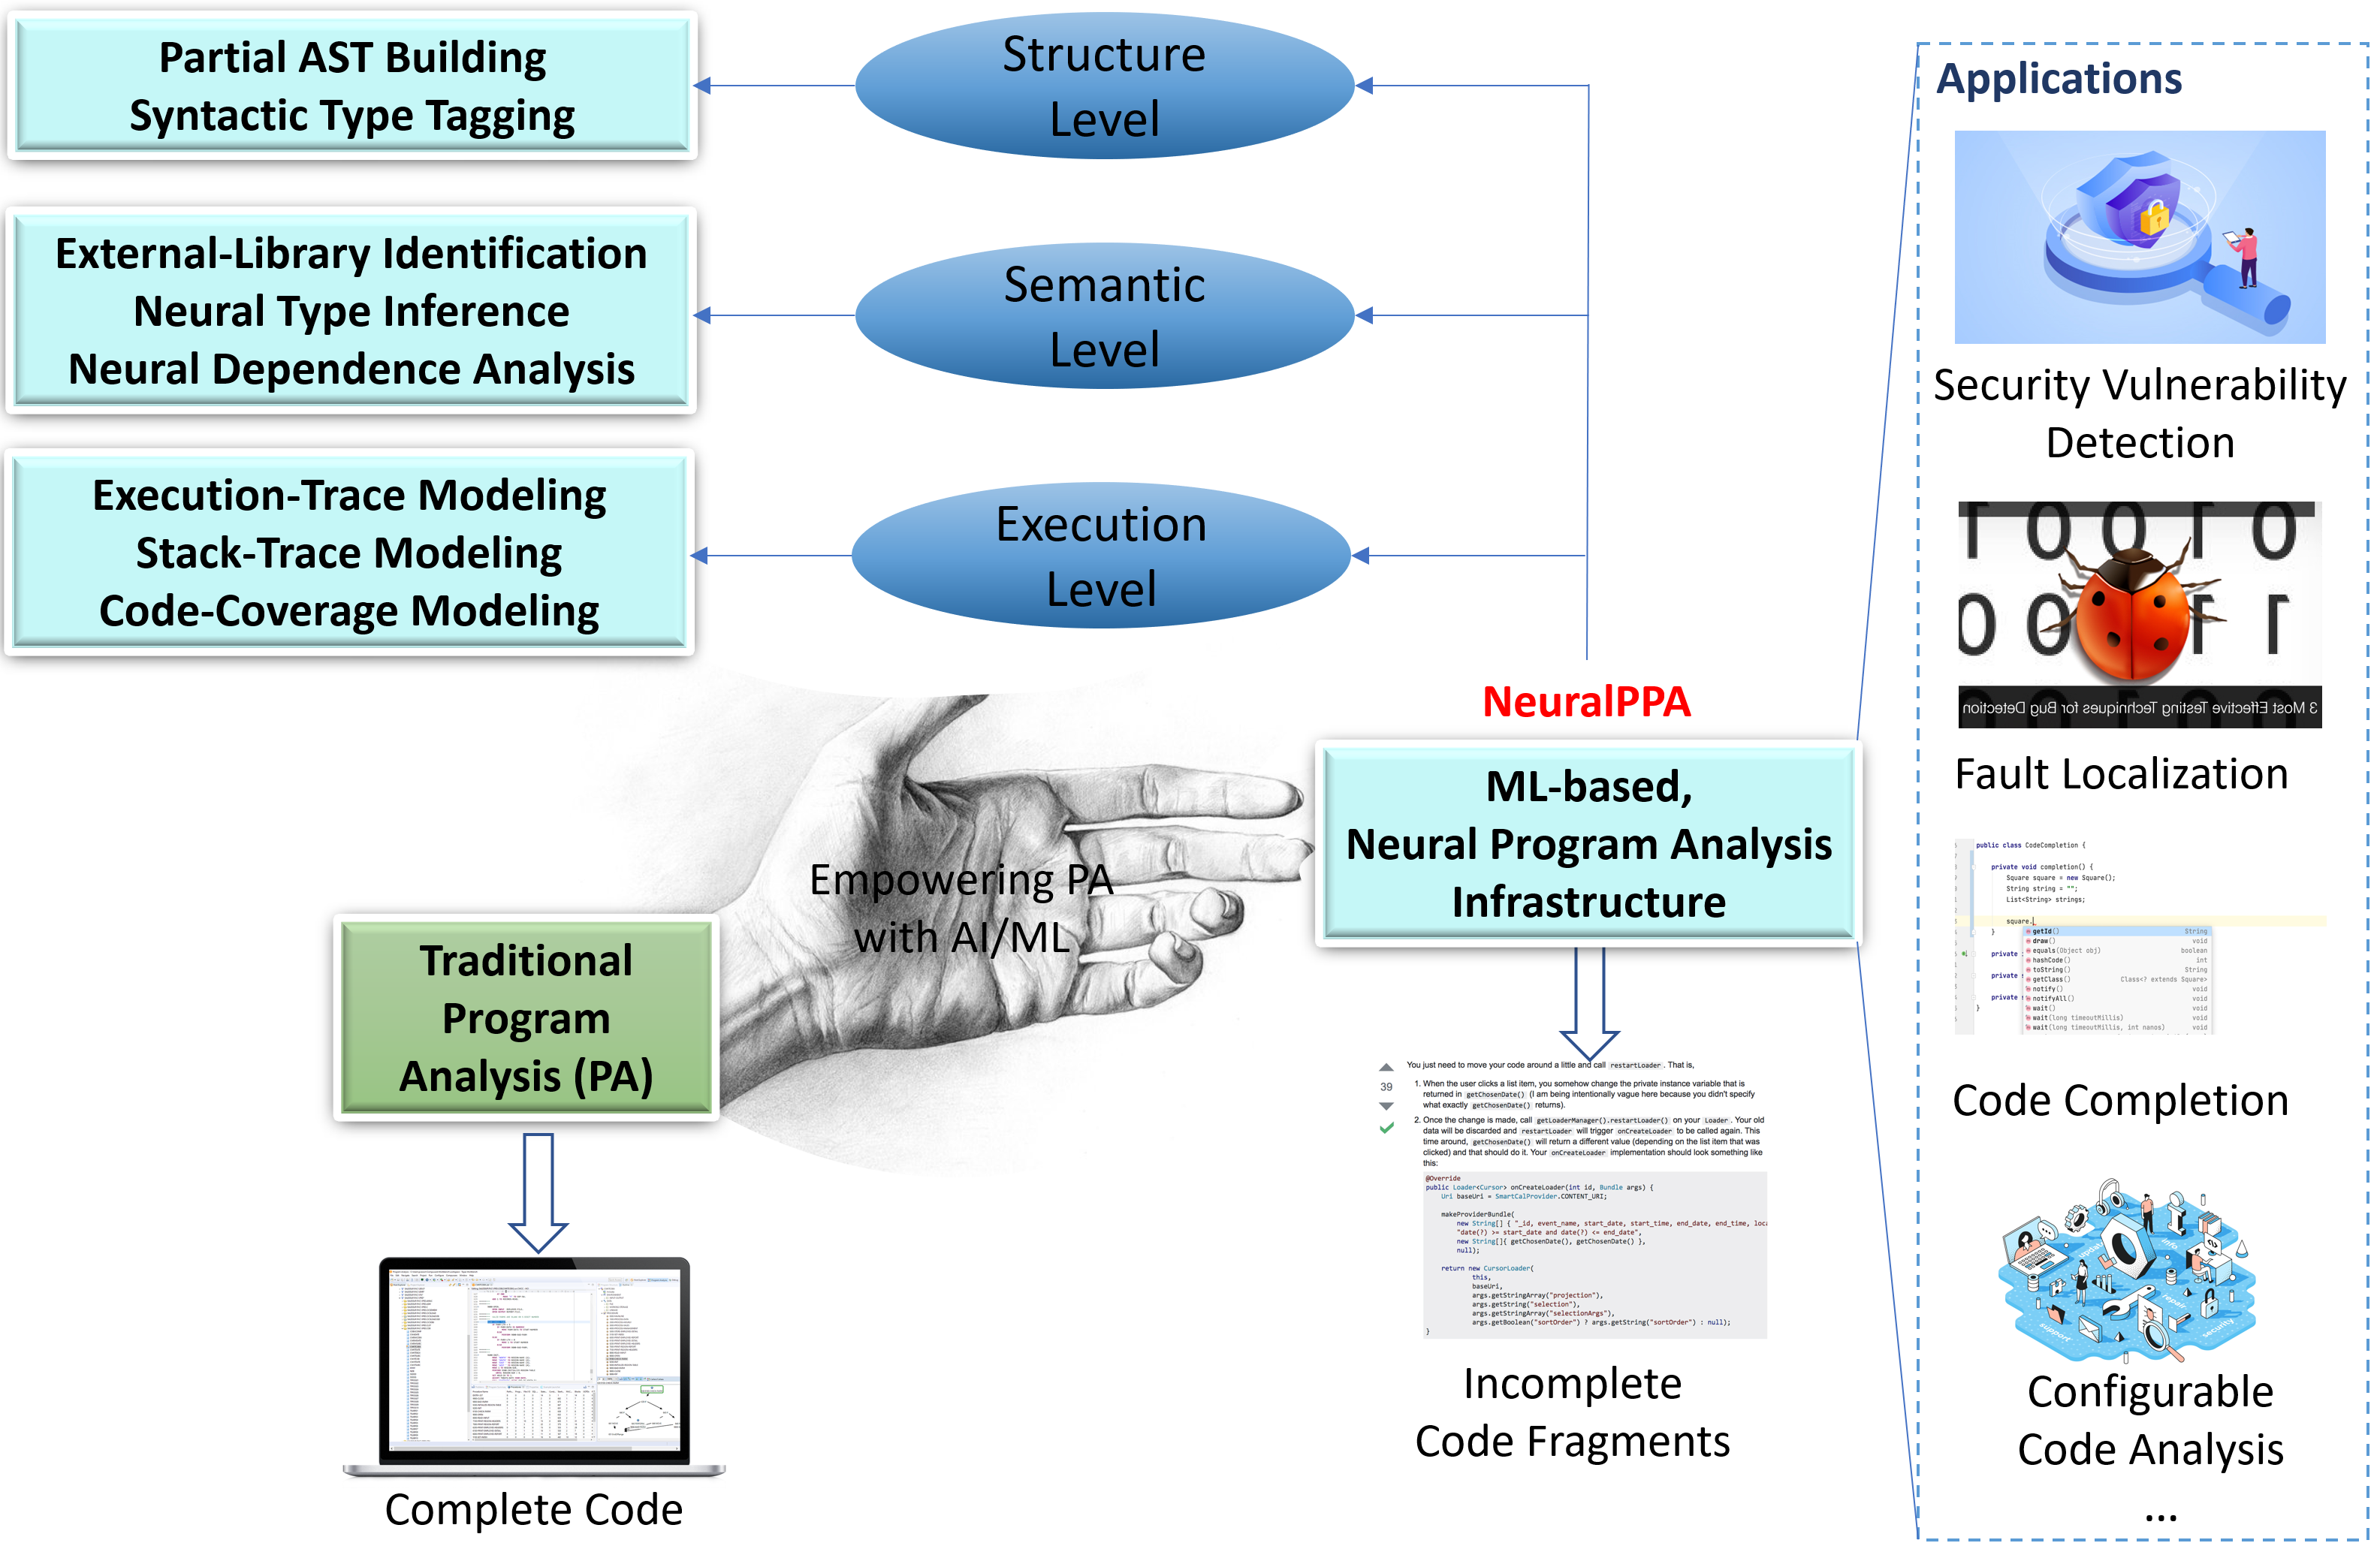
\includegraphics[width=0.9\textwidth]{graphs/neuralppa}
    \vspace{-12pt}
    \caption{{\tool}: Machine Learning-based Program Analysis Infrastructure}
    \label{fig:arch}
\end{figure}


While the state-of-the-art research and practice has been
well-established for the analysis of the entire programs, very little
research and knowledge has been achieved for partial program
analysis.
%
In this proposal, we set out to investigate and develop {\tool}, a
{\em \underline{Neural}-network-based \underline{P}artial
  \underline{P}rogram \underline{A}nalysis infrastructure}. We aim to
develop {\bf a scientific foundation, novel methodologies, frameworks,
  models, and algorithmic solutions for neural partial program
  analysis}. {\tool} {\bf enpowers program analysis (PA) with advanced
machine learning (ML) and artificial intelligence (AI) to enable the
program analysis on incomplete code fragments} (Figure~\ref{fig:arch}).
{\tool} will allow the constructions of the program analysis
techniques for partial code on which downstream software
engineering applications can be built.


In this work, our key philosophy is that {\em the analysis of
  partial code can be learned from the analysis of entire programs in
  the wealth of information from ultra-large-scale, open-source
  software repositories}.



Specifically, we draw our motivation for such a data-driven,
learning-based approach from the following. First, ultra-large-scale
software repositories, e.g. GitHub (7M+ projects) and SourceForge
(700k+ projects) contain an enormous collection of programs. These
repositories amount to 1,000,000,000+ lines of code, 10,000,000+
revision logs, and 3,000,000+ issue reports. This wealth of knowledge
is an excellent source for {\tool}. Hindle {\em et
  al.}~\cite{naturalness-icse12} have shown that code has high
repetitiveness and predictability, and can be captured well by
statistical models. Thus, we expect to build ML models to learn from
those repositories. Second, in an empirical study on the
repetitiveness, containment, and composability of PDGs in open-source
projects, the PI group~\cite{msr16} reported that among
17.5M PDGs with 1.6B PDG subgraphs, 14.3\% of the PDGs have all of
their subgraphs repeated across different projects. Furthermore, in
15.6\% of the PDGs, at least 90\% of their subgraphs are likely to
have appeared before in other projects. Thus, {\tool} could learn from
PDGs with complete program dependencies retrieved from existing code
repositories and derive the dependencies for the (partial) code
fragment under study. The PI group also reported a high repetitiveness
level for AST code structure in open-source
projects~\cite{icse15}. Finally, such a program analysis
infrastructure like {\tool} can be drawn from the spirit and successes
of the approaches in natural language processing (NLP). For example,
at the lexical level, the task of deriving the token types for source
code tokens could be analogous to the part-of-speech (PoS) tagging in
NLP. At the syntax level, the task of learning the syntactic structure
in AST of the partial code can be inspired by the approaches to build
parse trees for natural-language texts. At the semantic level, the
partial program dependence analysis infrastructure is similar in
spirit to the the neural network-based dependency parsing in NLP,
which learns the dependencies signifying the semantic relationships
between words in a sentence from text corpora.

Toward this theme, in our preliminary work, we developed DeepPDA, a neural
network-based partial program dependence analysis approach that learns
to derive the program dependencies for any code fragments (i.e., both
complete and incomplete). In our preliminary empirical evaluation, we
intrinsically evaluated it on Java and C/C++ programs. First, we
trained {\tool} on complete code. For testing, we treated each method
individually and chose a consecutive portion within the method to
predict the program dependencies, and compared them against the actual
dependencies. Overall, DeepPDA predicts CFG and PDG edges in Java
with an F-score of 94.29\%, and in C++ with an F-score of
92.46\%.
%
We also developed as an approach to derive the data
types of the variables in the code snippets. We treat the problem as
statistical machine translation from source code with partially
qualified names to source code with FQNs of the APIs. Our empirical
evaluation on real-world code and StackOverflow posts shows that our
technique achieves high accuracy with 97.6\% precision and 96.7\%
recall in deriving data types in code snippets.


In {\tool}, we propose the following thrusts of research
(Table~\ref{tab:milestones}):

\vspace{3pt}
\noindent \textbf{Thurst 1. Neural Structural Analysis Infrastructure
  \code{NeuralStruct}.} ({\em Section~\ref{}}) Source code has
well-defined structures and semantics. Thus, the basic infrastructure
in {\tool} is the neural structural analysis (\code{NeuralStruct})
component.  This component has two main tasks. First, it learns from
the syntactic structures of the complete code in the training dataset
collected from large-scale code repositories, to derive the abstract
syntax tree (AST) that best represents the syntactic structure of the
given partial code, i.e., with the highest likelihood/probability.
The traditional lexical analyzer still works for partial code due to
the independence nature of lexical tokens. The second task of this
component is to tag the code tokens with the types of the syntactic
units including the statement types (\code{if}, \code{for}, etc.),
variables, fields, methods, classes, etc. Both of the tasks can be
performed with our learning-based approaches in a dual-learning
manner.
  
\vspace{3pt}
\noindent \textbf{Thurst 2. Neural Semantic Analysis Infrastructure.}
({\em Section~\ref{}}) The basis components for several program
analysis techniques include the following:

1) the identification of the APIs of the external libraries in the
external references in the partial code: this is needed because the
partial code contains the undeclared reference and/or
declaration/reference ambiguity without explicit declaration of the
APIs in the external libraries.

2) the inference of the type information for the entities in the
partial code: due to the ambiguity in the declaration, the types of
the variables and statements are not always obviously defined. Thus,
the type inference is a basic service within {\tool}.

3) the inference of the program dependencies among the statements in
the partial code: several program analysis techniques are based on the
program dependencies, which are not always obtainable due to the
incompleteness of the given code fragment.

\vspace{3pt}
\noindent \textbf{Thurst 3. Neural Symbolic Execution Infrastructure.}
...

\vspace{3pt}
\noindent \textbf{Thurst 4. Neural Partial Program Analysis
  Applications.}  ({\em Section~\ref{}}) Our last thrust of research
is aimed to evaluate our basic partial program analysis infrastructure
in a few applications. We choose the following software engineering
applications: 1) software vulnerability detection for code snippets,
2) fault localization, and 3) code completion.

\vspace{3pt}
\noindent \textbf{Thurst ???. Neural Execution Analysis Infrastructure.}
({\em Section~\ref{}}) All the dynamic analysis techniques require the
analysis and understanding of the execution. However, for an
incomplete code, we first need to design a component that can wrap
around the given code fragment with the minimum code so that the code
fragment can be executed. When the code is executed, we also need the
approaches that represent the executed statements and their relations,
model the execution and stack traces, and model the code coverages
for an execution.


\begin{table*}[t]
	\vspace{-15pt}
\begin{center}
{\footnotesize{
\begin{tabular}{cc}
\begin{tabular}[t]{|p{0.2in}|p{2.95in}|} 
\hline
\multicolumn{2}{|>{\columncolor[gray]{0}}c|}{\textcolor{white}
{\bf Year 1 Project Milestones \& Deliverables}}\\
\hline 
\hline
\multicolumn{2}{|c|}{\bf T1. Neural Structure Analysis Infrastructure}\\
\hline
{\bf 1.1} & Neural Syntactic Type Tagging\\
{\bf 1.2} & Neural Partial AST Building\\
{\bf 1.3} & Evaluation of the components\\
\hline
\hline
\multicolumn{2}{|c|}{\bf T2. Neural Semantic Analysis Infrastructure}\\ 
\hline
{\bf 2.1} & External-Library Identification\\
\hline
%\hline
%\multicolumn{2}{|c|}{\bf Integrate Code Synthesis into Tools}\\
%\hline
%{\bf 1.5} & \goalOneFour.\\
%\hline
\multicolumn{2}{c}{}
\end{tabular}
&
\begin{tabular}[t]{|p{0.2in}|p{2.95in}|} \hline
\multicolumn{2}{|>{\columncolor[gray]{0}}c|}{\textcolor{white}
{\bf Year 2 Project Milestones \& Deliverables}}\\
\hline 
\hline
\multicolumn{2}{|c|}{\bf T2. Neural Semantic Analysis Infrastructure}\\
\hline
{\bf 2.2} & Neural Type Inference\\
{\bf 2.3} & Neural Dependence Analysis\\
%{\bf 2.3} & Integrate Evaluation Framework into Design Environment\\
%{\bf 2.4} & Evaluate CRL Framework with Existing Models\\
%{\bf 2.3} & \goalTwoThree.\\

\hline
\hline
\multicolumn{2}{|c|}{\bf T3. Neural Execution Analysis}\\ 
\hline
%{\bf 3.1} & Design New Code Representations and Learning Models.\\
{\bf 3.1} & Neural Execution-Trace Modeling\\
%{\bf 2.4} & Advance FL and RT-CI Approaches.\\
%{\bf 2.5} & Advance Regression Testing in CI Approaches.\\
%{\bf 2.5} & Advance APR Approaches with Framework.\\
\hline
%\hline
%\multicolumn{2}{|c|}{\bf Community Involvement: Capacity Building}\\
%\hline
%{\bf 2.4} & \goalTwoFour.\\
%{\bf 2.5} & \goalTwoFive.\\
%{\bf 2.6} & \goalTwoSix.\\
%\hline
\multicolumn{2}{c}{}
\end{tabular}
\end{tabular}\\
\vspace*{-.3cm}
\begin{tabular}{c}\hline
\multicolumn{1}{|>{\centering\columncolor[gray]{0}}p{6.44in}|}{\textcolor{white}
{\bf Year 3 Project Milestones \& Deliverables}}\\
\hline
\end{tabular}\\
\vspace*{-.2cm}
\begin{tabular}{cc}
\begin{tabular}[t]{|p{0.2in}|p{2.95in}|}
\hline
\multicolumn{2}{|c|}{\bf T3. Neural Execution Analysis}\\
\hline
{\bf 3.2} & Neural Stack Trace Modeling\\
{\bf 3.3} & Neural Code Coverage Modeling\\

%{\bf 3.3} & Testing on Models in IDE tools.\\
\hline
%\hline
%\multicolumn{2}{|c|}{\bf \goalTwo}\\ 
%\hline
%{\bf 3.3} & \goalThreeThree.\\
%\hline
\multicolumn{2}{c}{}
\end{tabular}
&
\begin{tabular}[t]{|p{0.2in}|p{2.95in}|}
\hline
\multicolumn{2}{|c|}{\bf T4. Neural Partial Program Analysis Applications}\\
\hline
%{\bf 3.1} & Design New Code Representations\\

{\bf 4.1} & Security Vulnerablity Detection with {\tool}\\
{\bf 4.2} & Fault Localization and Completion with {\tool}\\

\hline
\multicolumn{2}{c}{}
\end{tabular}
\end{tabular}
\vspace{-15pt}
}}
\end{center}
\vspace*{-.3in}
%\caption{Tasks and Milestones. (Rep. = Representation)}
\caption{The 3-year schedule of Thrusts, Tasks, and Milestones of this proposal.}
%the schedule of Thrusts, Tasks, and Milestones of this proposal.
%\vspace{-10pt}
\label{tab:milestones}
\vspace{-10pt}
\end{table*}
%






%\subsection{Significance of This Proposed Project: NSF Merit Criteria}

\section{Intellectual Merits}

The results of this project will advance the state-of-the-art
knowledge and scientific foundations in both program analysis and
machine learning. They are transformative and directly help improve
software quality with novel program analysis and vulnerability
detection tools.

\noindent \underline{{\bf Advance the state-of-the-art knowledge and
    understanding}}. Neural program analysis infrastructure in Thrusts
1--3 will advance the body of knowledge and theoretical foundations
for machine learning and AI for code. Thrust 4 will help advance the
practical tools for software security and engineering.

\noindent \underline{{\bf Scientific foundation, creative/original
    research}}. This project will provide a scientific
foundation (novel concepts, representations, algorithms, models,
and tools) (1) to enable the analysis on partial code, (2) to empower
the program analysis techniques on both (in)complete code,
and (3) to enable the applications of program analysis on incomplete
code such as vulnerability detection on code snippets, code
completion, etc.

\section{Broader Impacts}

\underline{{\bf (1) Transformative and benefits to society}}. Our
results will be transformative and directly benefit to our society.
They will lead to increasing developers' productivity, software
quality \& reliability.  Our validation involves students and
professionals, promoting teaching, training, and learning of both {\bf
  program analysis} and {\bf machine learning} techniques that
have wide impacts in industry and academic communities.

\noindent\underline{{\bf (2) Foster other related research
    activities}}. Our results will foster {\em research activities in
  related fields of {\bf deep learning} and {\bf software
    security}}. This project will produce theoretical concepts and
techniques that are novel even in deep learning, e.g., novel neural
networks to model and learn for code. The applications of our neural
program analysis in software engineering applications will advance
software security and reliability.

%The collected {\bf large scale bug\&fix corpus} will be useful for
%software quality and reliability research.
%Innovations in CRL could be used to {\bf advance other SE tasks}. We
%will also develop {\bf novel DL-based bug detect-fix} approaches.


\noindent\underline{{\bf (3) Education, dissemination, and broader participation}} (Section~\ref{edu}). The
research will enhance the infrastructure for teaching/research via
tools and data sets for use by students and practitioners, and for
enhancement by researchers. We will provide related learning
modules for educators as well. It will include outreach activities for
undergraduate students, underrepresented groups, minorities, and women
in science.
%contribute novel
%teaching modules to our curriculum.
%Details will be presented in Section~\ref{edu}


\iffalse
\begin{itemize}
	\vspace{-5pt}
\itemsep-0.2em 
  \item {\bf Transformative and benefits to society}. Our 
    results will be transformative and directly benefit to our
    society. 
    They will lead to increasing developers' productivity
    and software quality \& reliability. 
    Our validation involves students and
    professionals, promoting teaching, training, and learning of bug detecting and fixing techniques that have wide impacts 
    in industry and academic communities.

%report

  \item {\bf Foster other research activities}. Our results will
    foster research activities in related fields of deep learning and
    software quality. 
    This project will produce theoretical
    concepts and techniques that are novel even in deep learning, e.g.,
    novel neural networks for modeling and learning code. 
    The collected large scale bug fixing corpus will be useful for software quality and reliability research in general.
    %e.g.,   code transformation. 
%    This project will also advance
%    the state-of-the-art research in large-scale program analysis with
%    deep neural network models.

%The representation for software security vulnerabili will be useful in
%research on software security, malware detection, vulnerability
%reports, and automatic security patching.


  \item {\bf Education, dissemination, and broader participation}.
  The research will enhance the infrastructure for teaching and
  research by providing tools and data sets for use by students and
  practitioners, and for enhancement by other researchers. We will
  provide related learning modules for educators as well. It will
  contribute novel teaching modules to our curriculum. Details will be
  presented in Section~\ref{edu}

%Details are in Section 4.

\end{itemize}
\fi

%\input{sections/ccf-intro-new.tex}
%\input{example}
%\input{background}
\section{\color{red}{Related Work}}
%Our project is closely related to the following research literature: 
\textbf{Code Representation Learning (CRL).}  The recent success in
machine learning has lead to strong interests in applying machine
learning, especially deep learning, to programming language (PL) and
software engineering (SE) tasks, such as automated correction for
syntax errors~\cite{Bhatia-2016}, fuzz testing~\cite{Patra-2016},
program synthesis~\cite{Amodio-2017}, code
clones~\cite{White-2016,Smith-2009,Li-2017}, program
summarization~\cite{Allamanis-2016,Mou-2014}, code
similarity~\cite{Zhao-2018,Alon-2018}, probabilistic model for
code~\cite{Bielik-2016}, and path-based code representation,
e.g., Code2Vec~\cite{Alon-2018} and Code2Seq~\cite{alon2018code2seq}. 

%In the above PL and SE tasks, 
%All approaches learn code
%representations using different program properties. 
%Although not proposed for detecting bugs, they
%still very relevant to our proposal. %as one important step of our approach is to learn bug detection specialized code representation.

%Different from the existing CRL approaches, in our initial
%study~\cite{yioopsla19}, we conducted the CRL using the AST, DFG, PDG,
%and different attention-based neural networks. Our results show that
%our CRL is more suitable for detecting bugs than the existing baselines.


\textbf{Bug Detection.}
%Many techniques have been developed for rule-based and learning-based bug detection. 
Some existing rule-based bug detection approaches,
such as
\cite{Bian-2018,Jin-2012,Olivo-2015,Engler-2001,Cole-2006,Toman-2017},
are unsupervised. However, new rules are needed to
define to detect new types of bugs, e.g., FindBugs~\cite{Hovemeyer-2007} and NAR-miner~\cite{Bian-2018}.
%
%The most state-of-the-art \textit{rule-based} tool is NAR-miner~\cite{Bian-2018} that extracts
%negative code rules to detect bugs. %, instead of positive code rules. 
%Our initial results show the NAR-miner has a
%high false positive rate, i.e., 52\%, which make them
%impractical for daily use. 
%that it only costs NAR-miner 1 minute to perform bug detection on
%a project. However the mining-based approaches mainly suffer the
%problem of high false positive (FP) rates, such as the NAR-miner has a
%high FP rate, i.e., 52\% in the cross-project setting, which make them
%impractical for daily use. 
%When comparing our approach with the existing state-of-the art rule-based and mining approaches, the main differences are as follows. First, we consider the relations among paths from different methods for detecting cross-method bugs. However,
%they normally work on individual methods and cannot work well on the
%cross-method bugs. Second, our approach covers path information in an
%AST in order to detect very detailed bugs in each method, while the
%they often consider the important rules and may miss some information
%outside of their rules.
To overcome the pre-defined rules, the mining-based approaches, e.g.,~\cite{Bian-2018,Jin-2012,Olivo-2015,Engler-2001,Cole-2006,Toman-2017,Li-2005}, were proposed to mine implicitly programming rules from source code using data mining techniques. 
%Typically, this type
%of approaches extracts implicitly programming
%rules from program source code using data mining approaches
%(e.g., mining frequent itemsets or sub-graphs) and detects
%violations of the extracted rules as potential bugs. 
They still have a key limitation in a very high false positive rate
due to the fact that they cannot distinguish the cases of incorrect
code versus infrequent/rare code.  There exist DL-based
approaches~\cite{Pradel-2018,Wang-2016b} and traditional ML
techniques~\cite{Engler-2001,Li-2005,Wasylkowski-2017,
  Wang-2016b,Wang-2016,Liang-2016}.
%For example, 
%the Bugram \cite{Wang-2016} uses n-gram models to rank the methods and then picks the top-ranked methods as buggy methods.
%DeepBugs~\cite{Pradel-2018} uses deep learning techniques to propose
%a name-based bug detector.  
DL-based approaches are still limited to detect bugs in individual
methods.
%without investigating the dependencies among different yet
%relevant methods.

%$Due to that, they have high false positive rates, making them less
%practical in the daily use of software developers.
%In practice,
%there exist several cases that bugs occur across more than one
%method. That is, to decide whether a given method is buggy or not, a model
%needs to consider other methods that have data and/or control
%dependencies with the method under investigation. 
%Due to that, the
%existing DL-based approaches have high false positive
%rates, making them less practical in the daily use. % of software
%developers. 
%For example, DeepBugs~\cite{Pradel-2018} is reported to have a high false positive rate of 32\%. That is, approximately one out of 3 reported bugs is not a true bug, thus, wasting much developers' efforts. 
%Our study~\cite{yioopsla19i} also showed a false positive rate of 41\% for DeepBugs on our collected dataset.


%In this paper, our approach is also using the deep learning techniques to train the models and
%classify methods into buggy or non-buggy. Our approach is different
%from the existing learning-based approaches in the following ways.
%First, like the rule-based approaches, the existing learning-based
%approaches do not consider the relations among paths across multiple
%methods. In our code representation learning step, we model the
%relations among paths from different methods using the dependencies of
%entities in the PDG and DFG, in addition to the AST nodes of a path.
%Second, our approach uses long paths of an AST to cover all of the AST
%nodes for representing local context, while other existing approaches
%often use part of method information to detect bugs, such as
%name-based identifier representation and frequent $n$-grams. Our
%results show that our approach can outperform all of the
%studied baselines.


%\textit{Machine learning-based bug	detection~\cite{Wasylkowski-2017,Wang-2016b,Wang-2016,Pradel-2018}.}
%With the advances of machine learning (ML) and especially deep
%learning models, several approaches have been proposed to learn from
%previously known and reported bugs and fixes to detect bugs in the
%new code. While the ML-based bug detection models~\cite{Nam-2015}
%rely on feature selections, the deep learning-based
%ones~\cite{Pradel-2018,Wang-2016b} take advantages of the capability
%to learn the important features from the training data for bug
%detection. 


\textbf{Fault Localization and Regression Testing.}
Spectrum-based Fault Localization (SBFL)~\cite{zhang2011localizing, abreu2007accuracy, jones2005empirical, abreu2006evaluation, naish2011model, wong2007effective, liblit2005scalable, lucia2014extended, keller2017critical} has been intensively studied in the literature, e.g., Ochiai \cite{abreu2006evaluation} and Jaccard \cite{abreu2007accuracy}. 
%Tarantula \cite{jones2001visualization}, SBI \cite{liblit2005scalable}, Ochiai \cite{abreu2006evaluation} and Jaccard \cite{abreu2007accuracy}.  
%they share the same basic insight, i.e., code elements mainly executed by failed tests are more suspicious. 
Mutation-based Fault Localization (MBFL)~\cite{moon2014ask, zhang2013injecting,budd1981mutation, zhang2010test, musco2017large} aims to additionally consider impact information for fault localization, e.g., Metallaxis \cite{papadakis2012using, papadakis2015metallaxis} and MUSE \cite{moon2014ask}.
%Since code elements covered by failed/passed tests may not have any impact on the corresponding test outcomes, e.g., Metallaxis \cite{papadakis2012using, papadakis2015metallaxis} and MUSE \cite{moon2014ask}.
%typical MBFL techniques
%use mutation testing \cite{budd1981mutation, zhang2010test, musco2017large} to simulate the impact of each
%code element for more precise fault localization, e.g., Metallaxis \cite{papadakis2012using, papadakis2015metallaxis} and MUSE \cite{moon2014ask}.
%The first general MBFL technique, Metallaxis [24, 26] is based on the
%following intuition: if one mutant has impacts on failed tests (e.g.,
%the tests outcomes change after mutation), its corresponding code
%element may have caused the test failures
%
%The more recent MUSE [23] technique has similar insights: (1)
%mutating faulty elements may cause more failed tests to pass than
%mutating correct elements; (2) mutating correct elements may
%cause more passed tests to fail than mutating faulty elements.
%
%Learning-to-Rank (LtR) has been used to improve fault localization~\cite{b2016learning, xuan2014learning, li2017transforming, sohn2017fluccs}.
%MULTRIC \cite{xuan2014learning} combines different suspiciousness values from SBFL. Some work combines SBFL suspiciousness values with
%other information, e.g., program invariant \cite{b2016learning} and source code complexity information \cite{sohn2017fluccs}, for more effective LtR fault localization. 
%TraPT \cite{li2017transforming} combines suspiciousness values from both SBFL and MBFL. 
Neural networks have been applied to fault
localization~\cite{zheng2016fault, briand2007using, zhang2017deep,
  wong2009bp}. However, they mainly work on the test coverage
information, which has clear limitations (e.g., it cannot distinguish
elements accidentally executed by failed tests and the actual faulty
elements)~\cite{li2017transforming}. DeepFL~\cite{DeepFL},
deep-learning based, was proposed to improve method-level FL, and it
improves the learning-to-rank FL approach,
TraPT~\cite{TraPT}. Extensive research has been on test case selection and prioritization in regression testing (RT), e.g., coverage-based~\cite{di2015coverage}, search-based~\cite{de2011multi,yu2010time}, historical tests~\cite{kim2002history,marijan2013test,noor2015similarity,park2008historical}, code dependencies~\cite{gligoric2015ekstazi} and information retrieval~\cite{kwon2014test,saha2015information}. 
%RT in Continuous Integration (CI) differs from the traditional RT as 
However, most techniques cannot be applied at the scale of modern Continuous Integration (CI) practices~\cite{elbaum2014techniques} that require frequent commits to the shared code base and cause the cost of continuous RT escalate dramatically~\cite{memon2017taming}. For example, coverage information may be infeasible and imprecise to collect at large scale and in quick cycles and code changes~\cite{elbaum2014techniques,haghighatkhah2018test,hemmati2015prioritizing,yu2018study}. 
Recently, RT in CI has been investigated, e.g.,~\cite{elbaum2014techniques,gligoric2015practical,yu2018study,jiang2009adaptive,henard2016comparing}. 
However, existing approaches, e.g.,~\cite{bertolino2020learning,spieker2017reinforcement} are still limited in accuracy and scalability as they lack the learning of deep features of test cases and source code and their relations. 
%Moreover, very little research has been devoted to investigating deep learning for RT in CI. 


\textbf{Automated Program Repair.}
%The earlier approaches for automated program repair (APR) aim to derive {\em similar fixes for similar source code}. Ray and Kim~\cite{ray-fse12} automatically detect similar fixes for similar code that are ported or branched out. FixWizard~\cite{icse10} automatically derives {\em the fixes for similar code} that were cloned from one place to another.
APR approaches have explored search-based SE to tackle more general
types of bugs, e.g., GenProg~\cite{le2011genprog},
RSRepair~\cite{qi2014strength}, MutRepair~\cite{martinez2016astor},
PAR~\cite{kim2013automatic}, and SPR~\cite{long2015staged}.
%\cite{le2011genprog,qi2014strength,LeGoues-icse12,martinez2016astor}.
%A search strategy is performed in the space of potential solutions
%produced by several operators that mutate the buggy code. Then, the
%test cases and/or program verification are applied to select the
%better candidate fixes~\cite{smith2015cure}. 
%Smith et al.~\cite{smith2015cure} showed that 
%However, these
%approaches tend to overfit on test cases, by generating incorrect
%patches that pass the test cases, mostly by deleting functionalities~\cite{smith2015cure}.
%
%GenProg~\cite{le2011genprog} uses genetic search on repair mutations
%and works at statement-level by inserting, removing or replacing a
%statement taken from other parts of the same
%program. RSRepair~\cite{qi2014strength} fixes buggy programs with
%random search to guide the patch generation
%process. MutRepair~\cite{martinez2016astor} attempts to generate
%patches by applying mutation operators on suspicious if-condition
%statements. 
%PAR~\cite{kim2013automatic} is based on {\bf fixing templates} that
%were manually extracted from 60,000 human-written patches. 
%Later
%studies (e.g., \cite{le2016history}) showed that the six templates in PAR~\cite{kim2013automatic} could fix only a few bugs in Defects4J. 
%Anti-patterns were integrated into search-based APR tools~\cite{tan2016anti}
%Anti-patterns were integrated into search-based APR tools, e.g., GenProg~\cite{le2011genprog} and SPR~\cite{long2015staged}), to help alleviate the problem of incorrect or incomplete fixes.
%Theses search-based approaches rely much on the quality of mutation operations and the fixing patterns.
%
%\textbf{Hard-coded Rules based APR.}  Some existing APR techniques are
%mostly based on hard-coded rules and operators, defined by human
%experts, used to generate potential patches obtained with mutation
%operators for a buggy code.  For example, GenProg~\cite{le2011genprog}
%uses genetic search on repair mutations and works at statement-level
%by inserting, removing or replacing a statement taken from other parts
%of the same program.  RSRepair~\cite{qi2014strength} tries to fix
%buggy programs with the same mutation operations in GenProg but uses
%random search to guide the patch generation process.
%MutRepair~\cite{martinez2016astor} attempts to generate patches by
%applying mutation operators on suspicious if-condition statements.
%These approaches have several limitations, rooted in the fact that
%they are based on handcrafted rules with limited scope (i.e., single
%statements, limited number of mutation operators, specific parts of
%expressions).  Moreover, Smith et al.~\cite{smith2015cure} showed that
%these approaches tend to overfit on test cases, by generating
%incorrect patches that pass the test cases, mostly by deleting
%functionalities.
%
%Kim et al.~\cite{kim2013automatic} initiated with PAR a milestone of APR based on fix templates that were manually extracted from 60,000 human-written patches. Later studies (e.g., \cite{le2016history}) have shown that the six templates used by PAR could fix only a few bugs in Defects4J.
%~\cite{tan2016anti} manually define a set of patterns for patch generating or filtering based on repair history.
%Anti-pattern~\cite{tan2016anti} integrated anti-patterns into two existing
%search-based automated program repair tools (namely, GenProg~\cite{le2011genprog} and SPR~\cite{long2015staged}) to help alleviate the problem of incorrect or incomplete fixes resulting from program repair.
%In their study, the anti-patterns are defined by themselves and limited
%to the control flow graph. Additionally, their anti-patterns are
%not meant to solve the problem of deriving better patches
%automatically, provide more precise repair hints to developers.
%In contrast to search-based approaches, other approaches have aimed to
%Another type of APR approaches {\bf mine and learn fixing patterns} from prior bug
%fixes~\cite{nguyen2013semfix,le2016history,liu2019avatar,kim2013automatic}, \textit{generating the state-of-the-art performance}. 
Another type of APR approaches {\bf mine and learn fixing patterns} from prior bug
fixes, \textit{generating the state-of-the-art performance}. The fixing patterns (or namely fixing templates) could be automatically
or semi-automatically mined, such as SemFix~\cite{nguyen2013semfix}, Prophet~\cite{long2016automatic}, Genesis~\cite{long2017automatic}, FixMiner~\cite{koyuncu2018fixminer}, HDRepair~\cite{le2016history}, CapGen~\cite{wen2018context}, SimFix~\cite{jiang2018shaping}, Avatar~\cite{liu2019avatar}, Nopol~\cite{Nopol}, ACS~\cite{ACS}, SketchFix~\cite{SketchFix}, ELIXIR~\cite{saha2017elixir}, and LSRepair~\cite{LSRepair}. Tbar~\cite{tbar-issta19} collects all existing fix-patterns.
%exploit fix patterns of static analysis
%violations as ingredients for patch generation.
%
%SemFix~\cite{nguyen2013semfix} uses symbolic execution and
%constraint solving to synthesize a patch. 
%Some studies extracts fix patterns from real human submitted patches or change histories, e.g., Prophet~\cite{long2016automatic}, Genesis~\cite{long2017automatic}, FixMiner~\cite{koyuncu2018fixminer}, and HDRepair~\cite{le2016history}.
%
%are based on the frequently
%occurred code change operations (e.g., Insert If- Statement) extracted from the patches in developer change histories.
 %
%Prophet~\cite{long2016automatic} learns code
%correctness models from a set of successful human patches. 
%Prophet learns a patch ranking model using machine learning algorithm based on
%existing patches. 
%Genesis~\cite{long2017automatic} can automatically
%infer patch generation transforms from developer submitted patches for APR.
%HDRepair~\cite{le2016history} repairs bugs by mining closed frequent bug fix patterns from
%graph-based representations of real bug fixes.
%ELIXIR~\cite{saha2017elixir} uses method call related templates from
%PAR with local variables, fields, or constants, to construct more
%expressive repair-expressions for synthesizing
%patches. 
%CapGen~\cite{wen2018context}, SimFix~\cite{jiang2018shaping},
%Avatar~\cite{liu2019avatar} exploit fix patterns of static analysis
%violations as ingredients for patch generation.
%\textbf{Fix Pattern Mining and Learning based APR.}  Another direction
%of APR approaches tend to automatically mine fix patterns or
%templates.  For example, SemFix~\cite{nguyen2013semfix} instead uses
%symbolic execution and constraint solving to synthesize a patch by
%replacing only the right-hand side of assignments or branch
%predicates.  Long and Rinard also proposed a patch generation system,
%Prophet~\cite{long2016automatic}, that learns code correctness models
%from a set of successful human patches. Prophet learns a patch ranking
%model using machine learning algorithm based on existing patches.
%They further proposed a new system, Genesis~\cite{long2017automatic},
%which can automatically infer patch generation transforms from
%developer submitted patches for automated program repair.  Motivated
%by PAR~\cite{kim2013automatic}, more effective automated program
%repair systems have been explored. HDRepair~\cite{le2016history} was
%proposed to repair bugs by mining closed frequent bug fix patterns
%from graph-based representations of real bug fixes.  Nevertheless, its
%fix patterns, except the fix templates from PAR, still limits the code
%change actions at abstract syntax tree (AST) node level, but are not
%specific for some types of bugs.  ELIXIR~\cite{saha2017elixir}
%aggressively uses method call related templates from PAR with local
%variables, fields, or constants, to construct more expressive
%repair-expressions that go into synthesizing patches.  More recently,
%CapGen~\cite{wen2018context}, SimFix~\cite{jiang2018shaping},
%FixMiner~\cite{koyuncu2018fixminer} are further proposed to fix bugs
%automatically based on the frequently occurred code change operations
%(e.g., Insert If- Statement) that are extracted from the patches in
%developer change histories.  Avatar~\cite{liu2019avatar} exploits fix
%patterns of static analysis violations as ingredients for patch
%generation So far however, pattern-based APR approaches focus on
%leveraging patches that developer applied to semantic bugs.
%\textbf{Deep Learning based APR:} 
Recently, deep learning has
been applied to APR for directly generating patches.  
%For example, DeepRepair~\cite{white2016deep} and DeepFix~\cite{gupta2017deepfix} learn similar source code for similar fixes.
%The first group
%of DL-based APR approaches {\em learn similar source code for similar fixes}. such as DeepRepair~\cite{white2016deep} and DeepFix~\cite{gupta2017deepfix}.
%DeepRepair
%leverages learned code similarities, captured with recursive
%auto-encoders~\cite{white2016deep}, to select the repair ingredients
%from code fragments that are similar to the buggy code.
%DeepFix~\cite{gupta2017deepfix} learns the syntax rules and is
%evaluated on syntax errors.
Some work treats APR as a {\em statistical machine translation} translating the buggy code to the fixed
code. A natural thinking is to use neural translation models to learn to recommend fixes, such as Ratchet~\cite{hata2018learning}, Tufano {\em et al.}~\cite{tufano2018empirical}, SequenceR~\cite{chen2018sequencer}, Tufano {\em et al.}~\cite{tufano2019learning}, CoCoNuT~\cite{lutellier2020coconut} and CODIT~\cite{CODIT}. 


%learns code edits with encoding code structures in
%an NMT model to recommend fixes. 

%learn code changes using S2S NMT with code abstractions and keyword
%replacing.

%use sequence-to-sequence (S2S)
%translation. %They use neural network machine translation (NMT) with attention-based Encoder-Decoder, and different code abstractions to
%generate patches, while 
%SequenceR~\cite{chen2018sequencer} uses S2S with a copy mechanism~\cite{see2017get}.
%CODIT~\cite{codit} learns code edits with encoding code structures in
%an NMT model to recommend fixes. 
%The comparison with these NMT-based
%APR approaches is provided in the introduction. 
%Tufano {\em
%	et al.}~\cite{tufano2019learning} learn code changes using S2S NMT with code abstractions and keyword
%replacing. 
%Despite of treating the APR as code transformation learning
%problem, their approach takes entire method as a context for a bug.
%Thus, it has too much noise, leading to lower effectiveness than our initial approach {\tool}~\cite{icse_fl}.

%than {\tool}. In other words, the treatment of context from {\tool} helps improve over their model.



\section{Thrust 1. Neural Structural Analysis Infrastructure}
\label{sec:thrust1}

\subsection{Planned Work on Syntactic Type Tagging and Partial AST Building}

\begin{wrapfigure}{r}{0.3\textwidth}
\begin{lstlisting}[basicstyle=\scriptsize\sffamily, stepnumber=1, numbers=left, numbersep=-6pt, framexleftmargin=0mm, framexrightmargin=0mm, language=Python, emph ={}]
    for element in item_list:
        if element > 0:
            value += 1
        else:
            selected = element
            break
\end{lstlisting}
\vspace{-0.1in}
\caption{Running example}
\label{run_ex}
\end{wrapfigure}

Let us consider the Python code snippet illustrated in Figure~\ref{run_ex} as a running example in this section. For the {\em syntactic type tagging} task (essentially a lexical classification), the goal is to tag the code tokens with their corresponding syntactic unit types like variables, fields, methods, classes, etc. For example, the code tokens in the running example would correspond to \code{FOR}, \code{LOCAL\_VARIABLE}, \code{IN}, ..., \code{=}, \code{LOCAL\_VARIABLE}, \code{BREAK}. 

Next, consider the task of building an abstract syntax tree for incomplete code. As mentioned in Section~\ref{sec:intro}, PPA~\cite{ppa08} accomplishes this task in a best-effort manner by means of a rule-based strategy that also involves eliminating tokens to achieve the desired intermediate representation. Thus, it is limited. Alternatively, we hypothesize that such a representation for partial programs can be learned from the ASTs of the whole programs in the existing code repositories. We plan to enable such a learning process by modeling the AST-building task as a {\em structured reordering} problem. First, during the training phase, we will collect pairs of source code tokens and their respective AST representations. Second, we will convert the ASTs into binary trees by: (a) merging a unary non-terminal node with its child to form a new non-terminal node; (b) adding a special {\em \#}-node to binarize the $n$-ary nodes~\cite{https://doi.org/10.48550/arxiv.2206.11719}. An example of the same is illustrated in Figure~\ref{fig:ast-bt-mapping}, where the sub-AST corresponding to lines 2--3 in the running example is binarized. Third, we will linearize the binary trees thus formed using a tree-traversal algorithm (inorder, pre-order, or post-order). Fourth, given sequence pairs of code tokens and corresponding linearized binary tree representations, we will carry out the structured reordering as a sequence-to-sequence neural machine translation (NMT) task. By design, the number of tokens on the target side in this NMT problem is the sum of the number of tokens in the program on the source side and the number of non-terminal tokens in the binarized AST.

\begin{figure}[h]
    \centering
    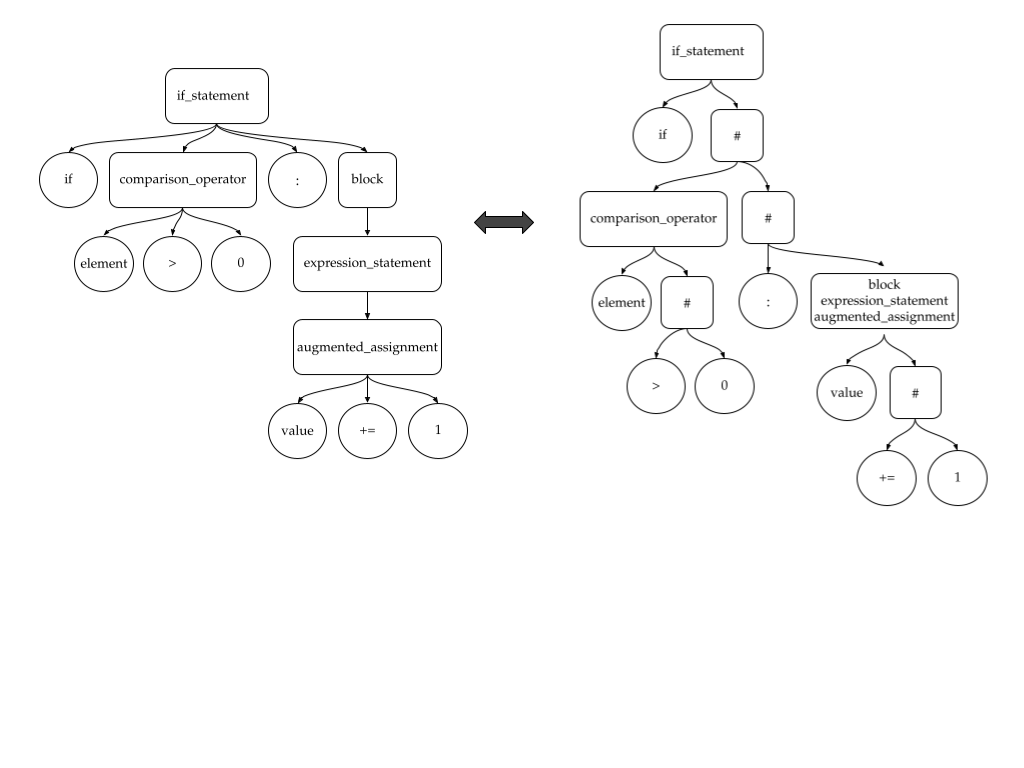
\includegraphics[width=\textwidth]{figures/ast-bt.png}
    \vspace{-130pt}
    \caption{Mapping an abstract syntax tree to its corresponding binary tree}
    \label{fig:ast-bt-mapping}
\end{figure}

For inference, one such trained NMT model can be leveraged to predict the linearized binary tree representation of the partial program under study.
The linearized binary tree representation can be used to reconstruct a unique binary tree (because of the one-to-one correspondence between them), and consequently the AST of the partial program. Moreover, the syntactic token types give information about a code token and its neighbors. Therefore, we plan to carry out both tasks, i.e., {\em syntactic-type tagging} and {\em partial AST-building} as a joint-learning process, which will help avoid error propagation from the former to the latter while benefiting each other. In addition, we will modify the decoding step in the NMT task to ensure that the ASTs thus generated for the partial programs are syntactically valid.


\section{Thurst 2. Neural Semantic Analysis Infrastructure}
\label{sec:thrust2}

\subsection{Planned Work on Type Inference for Partial Code}
\label{sec:statype}

\subsubsection{An Example of a StackOverflow Code Snippet}

\begin{wrapfigure}{l}{0.55\textwidth}
\begin{lstlisting}[basicstyle=\scriptsize\sffamily, stepnumber=1, numbers=left, numbersep=-6pt, framexleftmargin=0mm, framexrightmargin=0mm, language=Java, emph ={Event,sinkEvents,iframe,setEventListener,EventListener,StyleElement,Document,get,createStyleElement,setInnerText,resources,css,getText,getContentDocument,getHead,getBody,appendChild,ParagraphElement,createPElement,addClassName,whatever}]
    Event.sinkEvents(iframe, Event.ONLOAD);
    Event.setEventListener(iframe, new EventListener() {
        public void onBrowserEvent(Event event) {
            StyleElement style = Document.get().createStyleElement();
            style.setInnerText(resources.css().getText());
            iframe.getContentDocument().getHead().appendChild(style);

            ParagraphElement pEl = Document.get().createPElement();
            pEl.setInnerText("Hello World");
            pEl.addClassName(resources.css().getText());
            iframe.getContentDocument().getBody().appendChild(pEl);
        }
    });
\end{lstlisting}
\vspace{-0.1in}
\caption{StackOverflow post \#34595450 on GWT Widgets~\cite{soexample}}
\label{example}
\end{wrapfigure}

StackOverflow is a good resource of high quality code snippets that
show correct API usages. However, due to the discussion context and
the informal nature of the forum, code snippets rarely contain
sufficient declarations and references to fully-qualified names.

%This example illustrates three key challenges in resolving ype
%information.

Let us use a real-world example to illustrate the 
challenges in~resolving 
the fully qualified names (FQNs) 
for an SO code snippet. Figure~\ref{example} shows a
code snippet of an answer for an SO post
%\#34595450 
on Widgets in the GWT library. 

First, the snippets are not often embedded in methods or classes. In
Figure~\ref{example}, the code does not have an enclosing method or
class.

Second, they may refer to variables whose {\em declarations are not
  included}, and~their {\em identifiers are largely unqualified}. For
example, the variable \code{iframe} at lines 1, 2, 6, and 11 do not
have a declaration because the responder assumes that users would add
a declaration of type \code{IFrameElement} for \code{iframe} or add a
method call to the API \code{createIFrameElement} to get an object of
the type \code{IFrameElement}.
%
%\code{iframe} was declared earlier with the type \code{IFrameElement}
%a declaration of the type \code{IFrameElement} for \code{} 
%or an access to such an object by a prior call to
%\code{createIFrameElement}. 
%

Third, {\em the external references in code snippets are also often
  undeclared}. Specifically, code snippets frequently refer to
external types without specifying their FQNs since the
responder assumes that those FQNs could be implicitly understood in
the context of~the post.
%Tien
%
%assumes that users would add the required imported libraries when
%using the snippet in their programs in an IDE.
%
%
For example, the types \code{Event}, \code{EventListener},
\code{StyleElement}, \code{Document}, and \code{ParagraphElement} are
referenced by simple names only. Fourth, {\em name ambiguity occurs in
  the references to external libraries}. For example, the type
\code{EventListener} at line 2 is a common unqualified type name. In
this snippet, it refers to
\code{com.google.gwt.user.client.\-Event\-Listener}. However, it is
ambiguous with \code{java.util.EventListener} in JDK. Similarly, the
simple type name \code{Document} at line 4 is also popular
(\code{com.google.gwt.dom.client.Document},
\code{org.eclipse.jface.text.Document}, \code{org.w3c.dom.Document},
etc).
%Thus, if the code snippet is placed inside a class within an IDE, it
%will not be compiled due to missing \code{import} statements for
%needed packages.
%In fact, the phenomenon of 
In fact, external reference ambiguity is
popular~\cite{dagenais-icse12}.
%has been reported before.
%by Dagenais and Robillard~\cite{dagenais-icse12}: 89\% of method names
%in their study are ambiguous and on average, a method name has 13
%candidate FQNs.
%
%Subramanian {\em et al.}~\cite{liveapi14} reported that 
For example, the simple names \code{getId} and \code{Log} occur 27,434
and 284 times respectively in various Java libraries~\cite{liveapi14}.


%In a later version, it uses a dictionary of all the APIs of the
%libraries of interest. This is tedious to build a dictionary.


To address those ambiguities,
%in resolving the FQNs, for the elements in a code snippet,
existing approaches rely on rules and heuristics mainly from
program analysis. 
%
%ACE~\cite{rigby-icse13} focuses on resolving types for API names
%within texts via text analysis of the enclosing SO posts, thus, is
%inapplicable for this example.
%
RecoDoc~\cite{dagenais-icse12} uses heuristics in the partial program analysis tool,
PPA~\cite{dagenais-oopsla08}, 
%to apply heuristics on syntactic constructs to recover the declared
%types of certain expressions (\eg assignments). Unfortunately, 
however, in many cases, the heuristics help recover only partially
qualified names, due to much missing information. For example, at line
6, Figure~\ref{example}, the types of the receiver \code{iframe} and
method call \code{getContentDocument}, are not known. In contrast,
Baker~\cite{liveapi14} uses a dictionary of all the API names of
interest. Each API name has multiple candidates of FQNs. Baker
iteratively cuts off the candidates by overlapping the candidate lists
of API names in the same scopes in the code snippet. However, scoping
rule or other rules/heuristics are not always effective in incomplete
code snippets. In this example, lines 4--6 in Figure~\ref{example}
have only one scope with the popular API names having many potential
FQNs (\code{Document}, \code{getText}, \code{appendChild}). Moreover,
building and updating a dictionary of the APIs require
much~effort~\cite{dagenais-fse10}.


%{\em program analysis}, {\em text analysis}, or {\em deductive
%  analysis}, and/or the use of {\em an oracle of APIs of
%  interest}. 
%
%Specifically, partial program analysis (PPA)
%technique~\cite{dagenais-oopsla08} performs partial parsing and type
%resolution with several heuristics. PPA disambiguates the names by
%applying a set of heuristics on the syntactic constructs to recover
%the declared types of certain expressions in an incomplete code
%snippet. Unfortunately, in many cases, the heuristics help recover
%only partially qualified names, due to much missing information. For
%example, at line 6, the types of the receiver, method call, and
%arguments are not known.
%
%RecoDoc~\cite{dagenais-icse12} suffers the same issues since it uses
%PPA to link an API and documentation.
%
%ACE~\cite{rigby-icse13} focuses on resolving types for API names
%within texts via text analysis of the enclosing SO posts, thus, is
%inapplicable for this example. 
%Baker~\cite{liveapi14} uses a dictionary of all the API names of
%interest. Each API name has multiple candidates of FQNs.  Baker
%iteratively cuts off the candidates by overlapping the candidate lists
%of API names in the same scopes in the code snippet. However, scope
%rules are not always effective in incomplete code with few scopes or
%in popular names with many potential FQNs, \eg \code{Document},
%\code{getText}, \code{appendChild} on lines 4--6. Moreover, building
%and updating an oracle of the APIs require
%much~effort~\cite{dagenais-fse10}.

%=========================================================================
%To address those ambiguities in resolving the FQNs for the elements in
%a code snippet, existing approaches rely on {\em program analysis},
%{\em text analysis}, or {\em deductive analysis}, and/or the use of
%{\em an oracle of APIs of interest}.
%
%Specifically, partial program analysis (PPA)
%technique~\cite{dagenais-oopsla08} performs partial parsing and type
%resolution with several heuristics. PPA disambiguates the names by
%applying a set of heuristics on the syntactic constructs to recover
%the declared types of certain expressions in an incomplete code
%snippet. Unfortunately, in many cases, the heuristics help recover
%only partially qualified names, due to much missing information. For
%example, at line 1, the types of the receiver, method call, and
%arguments are not known. RecoDoc~\cite{dagenais-icse12} suffers the
%same issues since it uses PPA to link an API and documentation.
%ACE~\cite{rigby-icse13} focuses on resolving types for API names
%within texts via text analysis of the enclosing SO posts, thus, is
%inapplicable for this example. Baker~\cite{liveapi14} uses a
%dictionary of all the API names of interest. Each API name has
%multiple candidates of FQNs.  Baker iteratively cuts off the
%candidates by overlapping the candidate lists of API names in the same
%scopes in the code snippet. However, scope rules are not always
%effective in incomplete code with few scopes or in popular names with
%many potential FQNs, \eg \code{Document}, \code{getText},
%\code{appendChild} on lines 4--6. Moreover, building and updating an
%oracle of the APIs require much~effort~\cite{dagenais-fse10}.
%=======================================================================

%--------------------------------------------------------------
%To address those ambiguities in resolving the FQNs for the program
%elements in a code snippet, existing approaches rely on {\em program
%  analysis}, {\em text analysis}, and/or the use of {\em an oracle of
%  APIs of interest}. Specifically, partial program analysis (PPA)
%technique~\cite{dagenais-oopsla08} performs partial parsing and type
%resolution with several heuristics. PPA disambiguates the names by
%applying a set of heuristics on~the syntactic constructs to recover
%the declared types of certain expressions in an incomplete code
%snippet. Unfortunately, in many cases,~the heuristics help recover
%only partially qualified names, due to much missing information.  For
%example, at line 1, the types of the receiver, method call, and
%arguments are not known. RecoDoc~\cite{dagenais-icse12} suffers the
%same issues since it uses PPA to link an API and documentation. With
%context analysis, ACE~\cite{rigby-icse13} analyzes the API names by
%considering the {\em textual contexts} surrounding them in SO
%posts. However, it might not be always effective since the surrounding
%texts might not be sufficient and code snippets were not analyzed.
%Baker~\cite{liveapi14} uses a dictionary of all the API names in the
%libraries of interest. Each API name has multiple candidates of FQNs.
%Baker iteratively cuts off the candidates by overlapping the candidate
%lists of multiple names in the same scopes in the code
%snippet. However, scope rules are not always effective in incomplete
%code or in popular names with many potential FQNs, \eg
%\code{Document}, \code{getText}, \code{appendChild} on lines 4--6.
%Thus, after its process, the resulting API names from Baker still have
%multiple potential FQNs. Moreover, building and updating an oracle of
%the APIs require much~effort~\cite{dagenais-fse10}.
%-----------------------------------------------------------------

%is also time-consuming.

%
% many API elements have
% more than one potential fully qualified type names

%problem with oracle
%overlapping

%\vspace{-0.14in}
\subsubsection{Key Ideas in {\tool}}

%type references, method calls, and field references.

%resolve the simple names

As part of {\tool}, we will develop a technique to identify the FQNs for
the simple names of {\em variables, API classes, method calls, and
  field accesses} in a code snippet in online forums.
%
In our solution, we leverage two kinds of context in deriving FQNs for
API elements. 

The first one is the {\em type context} of API elements in a
large code corpus. 
%FINAL
%Hindle {\em et al.}~\cite{natural} has shown that software exhibits
%its naturalness: source code has a higher degree of regularity than
%English texts. We expect the same principle of naturalness of software
%to occur for the API elements in the API code usages. 
That is, in the API usages, the API elements including API classes,
method calls, and field accesses of software libraries do not occur
randomly. They appear regularly with certain other API elements due to
the intent of the libraries' designers to provide certain
functionality in API usages. For example, to manipulate style
information for a frame in GWT, at lines 4--6 in Figure~\ref{example},
a \code{StyleElement} in GWT could be created via a call to
\code{createStyleElement} of a \code{Document} object. Then, the style
is assigned with a name via \code{StyleElement.setInnerText} and
associated with an \code{IFrameElement} object. Those API elements of
those types repeatedly occur together because such tasks are provided
by the GWT library and intended via such API usages. Thus, if {\tool}
observes the API usages involving those API elements in a large corpus
of programs using GWT, it can use the context of the given code
snippet to derive the most likely FQNs for the APIs in the
snippet. For example, the context of the API names
\code{StyleElement}, \code{Document}, and \code{createStyleElement}
could give {\tool} a hint on the FQNs of the undeclared variable
\code{iframe}, the method calls \code{getContentDocument},
\code{appendChild}, and vice versa.
To learn the context, we rely on the basis of regularity with a large
corpus: the API elements regularly going together in API
usages have higher impact in deciding the FQNs than the less
regular~ones.

%ones that
%are project-specific and less likely to appear frequently~together.

%To learn the context, we rely on the basis of regularity with a large
%corpus containing the APIs of interest. That is, the API elements that
%regularly go together in API usages will have higher impact in
%deciding the FQNs than the ones that are project-specific and less
%likely to appear frequently~together. 

%
%For example, with a large corpus of programs using GWT, a model could
%learn that \code{com.google.gwt.user.client.Event.setEventListener}
%often goes with \code{com.google.gwt.user.client.Event.EventListener},
%and \code{com.google.\-gwt.user.client.Event.sinkEvents}.

The second context is called {\em resolution context} on how the types
of API names surrounding an API name have been resolved. The
undeclared/ambiguous references are expected to be disambiguated with
{\em the most likely FQNs with regard to the FQNs of the surrounding
  names}.
%
For example, at lines 3--4, when resolving \code{Event},
\code{StyleElement}, and \code{Document}, we could use an effective
search strategy to maintain the sequences of FQNs with the highest
probabilities. For \code{Event}, we have multiple candidates. However,
if we chose \code{com.google.gwt.user.client.Event} for \code{Event},
then based on their regularity, we could maintain the option
\code{com.google.gwt.dom.client.Document} for \code{Document}, with a
higher score than \code{org.w3c.dom.Document}. Finally, the sequence
with the highest score will be reported as the~result.

%Then, we use it to decide the type for the next API.

%with a large corpus of programs using GWT, a model could
%learn that \code{com.google.gwt.user.client.Event.setEventListener}
%often goes with \code{com.google.gwt.user.client.Event.EventListener},
%and \code{com.google.\-gwt.user.client.Event.sinkEvents}.



% ---- old ---
%In this work, to realize that philosophy, we use a data-driven
%approach with the two following key ideas:

%1) In the context of API usages, certain API elements need to be used
%together because they have to follow the API specifications. For
%example, with a large corpus of programs using GWT, a model could
%learn that \code{com.google.gwt.user.client.Event.setEventListener}
%often goes with \code{com.google.gwt.user.client.Event.EventListener},
%and \code{com.google.\-gwt.user.client.Event.sinkEvents}.
%To learn the contexts, we rely on the {\bf basis of regularity} with a
%large corpus containing the APIs of interest. That is, the API
%elements that regularly go together in API usages will have higher
%impact in deciding the FQNs than the ones that are project-specific
%and less likely to appear frequently~together.

%2) To narrow the candidate FQN list for an API name, we could use the
%{\bf context of its surrounding API names}. The undeclared/ambiguous
%references are expected to be disambiguated with the most likely FQNs
%with regard to the FQNs for surrounding names.
%------------------------------------------------------------

%
%\code{com.google.gwt.user.client.Event.sinkEvents} receives two
%arguments of the types \code{com.google.gwt.dom.client.Element} and
%\code{int}, and it often goes with
%\code{com.google.gwt.user.client.Event.setEventListener}, etc.
%
%For example, at line 1 of Figure~\ref{example}, even though we do not
%have the declaration of \code{iframe}, however, with the large corpus
%of open-source projects, the model could learn that the method
%\code{com.google.gwt.user.client.Event.sinkEvents} receives two
%arguments of the type \code{com.google.gwt.dom.client.Element} and
%\code{int}, and it often goes with
%\code{com.google.gwt.user.client.Event.setEventListener}.


%Tien
%\input{rules.tex}
%\input{smt-motiv}



%2) {\em Second}, because the translation takes into account {\bf the
%  context consisting of surrounding API elements/names}, the
%undeclared/ambiguous references will be disambiguated with the most
%likely FQNs with regard to the FQNs of their surrounding names.

%3) ambiguity: Third, not all the changes in the current context are useful in
%recommendation because they can be project-specific and considered
%as noise in the change patterns. Recent work [41] confirms
%that not all code changes are repetitive. To address this, we rely on
%the basis of consensus: given a large number of changes in many
%projects, the project-specific changes are less likely to appear frequently
%than the changes belonging to a higher-level intent pattern.
%-==> undeclared types


\subsection{Preliminary Work on Neural Program Dependence Analysis}
\label{sec:deeppda}

In the neural network-based dependency
parsing~\cite{chen-manning-2014-fast} in NLP, by projecting the words
into an embedding space, researchers successfully learn the semantic
relationships that model the dependencies between them. We can follow
suit to learn the control-flow and program dependencies between the
statements in programs as well. Moreover, given that the quality of
the statement embeddings determines the accurate prediction of the
program dependence relations, enhancing them by incorporating context
from both within and across the statements is crucial. Intra-statement
contextualization can help relay the local information within
individual statements globally. For example, such information can help
distinguishably identify the declaration and reference of the same
variable across  program statements. In contrast,
inter-statement contextualization helps learn the dependencies between
the statements in the context of the surrounding statements. Finally,
we aim to model the CFG/PDG construction as a pairwise dependence
decoding task, wherein the combination of all the predicted edges in
the statement pairs can be formalized as directed graphs, e.g., CFG/PDG.

\begin{figure*}[t]
\begin{center}
    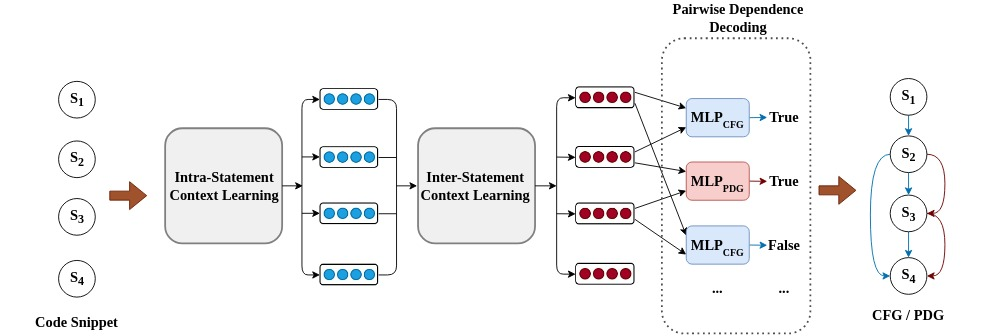
\includegraphics[width=0.9\textwidth]{model-abstract.jpg}
    \caption{Preliminary Design for \tool Model Infrastructure for Dependency Analysis for Partial Code}
    \label{fig:model}
    \vspace{-26pt}
\end{center}
\end{figure*}

%In Figure~\ref{fig:model}, we present a preliminary design of the
%general architecture of \tool model.

%Given that attention is the driver behind the now ubiquitous
%Transformers’~\cite{Vaswani-2017} success in efficiently learning
%representations for different entities in different contexts, we plan
%to make it the foundation of the context learning components in our
%model as well. Each is intended to learn different aspects of
%contextualization.

%\begin{figure*}
%    \centering
%  \subfloat[Intra-Statement Context Learning\label{fig:input_repr_a}]{%
%       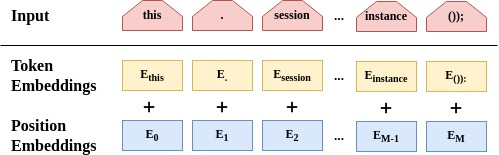
\includegraphics[width=0.45\linewidth]{figures/input_repr_tok.jpg}}
%  \hspace{0.25cm}
%  \subfloat[Inter-Statement Context Learning\label{fig:input_repr_b}]{%
%        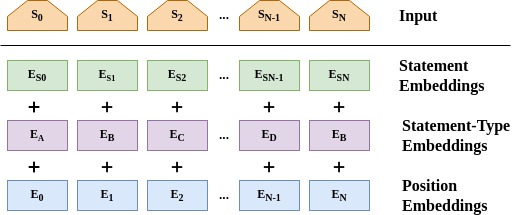
\includegraphics[width=0.45\linewidth]{figures/input_repr_stmt.jpg}}
%    \hfill
%  \caption{Input representations: (a) tokens in a statement are the sums of token embeddings, and (token) position embeddings; (b) statements in a snippet are the sums of statement embeddings, statement-type embeddings, and (statement) position~embeddings.}
%  \label{fig:input_repr}
%\end{figure*}


%\subsection{\bf Model Architecture}
%\label{sec:ppda_arch}

%As explained in Section~\ref{sec:overview}, better contextualization
%is the main idea behind \tool's design. Given that attention is the
%component in the ubiquitous Transformers'~\cite{Vaswani-2017} success
%in efficiently learning representations for different entities in
%different contexts, we chose to make it the foundation of our
%model. In brief, we realize \tool via a hierarchical, self-attention
%network (SAN)-based model architecture, where each sub-network is
%intended to capture different aspects of contextualization. Its
%details are as follows:

\vspace{2pt}
\subsubsection{{\bf Intra-Statement Context Learning (IntraS-CL)}}
\label{sec:ppda_arch_intra}
The syntactic and semantic knowledge of the code tokens within a
single statement must be made available globally to other statements
in a program to learn the inter-statement program dependencies
effectively. We enable this via a \textit{1-Layer} (i.e., $N_X$$=$$1$)
Self Attention Network (1L-SAN). The self-attention layer in an 1L-SAN
inputs $x_1, x_2, ..., x_n \in \mathbb{R}^d$, performs self-attention
once by projecting the inputs from all attention heads $\in
\mathbb{R}^{d_h}$ into the head dimension space $d_h$ via linear
transformations, and generate outputs $y_1, y_2, ..., y_n \in
\mathbb{R}^d$ which are linear combinations of the concatenated
attention head values. We use one attention head
(i.e., $h$$=$$1$) for the self-attention layer in 1L-SAN, and the size
of the input representations, i.e., $d$ is set to 512. Our experiments
revealed only a marginal performance gain by expanding the 1L-SAN to a
2L-SAN, which also came with high computational
overhead. Besides, increasing the number of attention heads did not
help either performance or interpretability. A more detailed analysis
on hyperparameters and subsequent
trade-offs is left to future~work.

\vspace{1pt} \underline{Input Representations}. For a program
comprising $N$ statements $s_1, s_2, ..., s_N$, \tool takes as input a
concatenation of $N$ sequences of $M$ tokens each, $\langle
t_1^{(1)}$, $t_2^{(1)}$.., $t_M^{(1)} \rangle$, ..., $\langle
t_1^{(N)}$, $t_2^{(N)}$.., $t_M^{(N)} \rangle$. Next, each token
sequence $\langle t_1^{(i)}$, $t_2^{(i)}$.., $t_M^{(i)} \rangle$ is
input to the 1L-SAN for intra-statement contextualization. Previous
works~\cite{radford2019language, liu2019roberta} have demonstrated
the~advantages of a byte-level Byte-Pair Encoding (BPE)-scheme for
tokenization. We follow suit to train a byte-level BPE tokenizer for
converting a given statement into a sequence of tokens. Here, $M$ is
the maximum number of tokens allowed in a statement.  For statements
with token sequences having ${<}M$ tokens, a special \textit{[PAD]}
token is appended. In contrast, token sequences having ${>}M$ tokens
are truncated to $M$ tokens.

%\vspace{1pt} \underline{Token Embeddings}. For all the words in the
%vocabulary $V$, we leverage a learnable embedding to learn and store
%their representations (i.e., $\mathbb{R}^{|V| \times d}$). Using this
%as a lookup table, token embeddings are retrieved for all the tokens
%generated by the tokenizer for a given statement.

%\vspace{1pt} \underline{Token Position Embeddings}. Attention
%mechanism in the self-attention layer is invariant to position
%information. However, this knowledge is key to understanding the
%sequential nature of code tokens in a statement. We enable this via
%learnable position encoding scheme, where a vector $\in \mathbb{R}^d$
%unique to each position is learned during the training process.

%\vspace{1pt} \underline{Statement (Output) Representations}. Input
%representations to the 1L-SAN corresponding to the tokens in a given
%statement are taken as the sums of the \textit{token embeddings}, and
%their \textit{position embeddings} (as in
%Fig.~\ref{fig:input_repr_a}). The 1L-SAN yields intra-statement
%contextualized token representations as its output, which are then
%averaged to retrieve the statement representation. Note that the token
%representations corresponding to the \textit{[PAD]} tokens are not
%considered for averaging. Such statement representations $u_i$ ($\in
%\mathbb{R}^d$) for all the statements $s_i \in s_1 ... s_N$ are then
%passed on for inter-statement contextualization.

\vspace{2pt}
\subsubsection{\bf Inter-Statement Context Learning (InterS-CL)}
The knowledge of surrounding statements in the context of a given
statement helps \tool model the dependencies between them better. We
enable this via a multi-layer bidirectional Transformer encoder based
on the work by Vaswani {\em et
  al.}~\cite{Vaswani-2017}. Owing to its common usage, we will omit
exhaustive background details on Transformers' model architecture and
will refer the readers to ~\cite{Vaswani-2017}. As shown in
Fig.~\ref{fig:model}, we denote the number of layers in the
Transformer encoder by $N_Y$, which we set to 6. We employ 4 attention
heads, i.e., $h$$=$$4$ to increase parallelization (since
$d_h$$=$$\frac{d}{h}$, i.e., $d_h$$=$$128$) and learn different
aspects of the syntactic and semantic structure in the statements,
while still being interpretable. We also set the feed-forward module
size to be 4 times that of the size of the input representations $d$,
i.e., 2048. Overall, Transformer in InterS-CL phase inputs
local context-aware statement representations $u_i \in \mathbb{R}^d$
for all statements $s_i$ in a given program, and outputs statement
representations $v_i \in \mathbb{R}^d$ that are both local and global
context-aware.

\vspace{1pt} \underline{Statement Input Representations}. For all the
statements $s_i$, statement embeddings (i.e., $u_i \in
\mathbb{R}^d$) are obtained from the 1L-SAN in the IntraS-CL phase.
$N$ is the maximum number of statements in a method in the dataset. If
a given program has less than $N$ statements,
zero vectors ($\in \mathbb{R}^d$) are padded to the inputs.

%\vspace{1pt} \underline{Statement Position Embeddings}. To make our
%model under\-stand the sequential nature of statements in a program,
%as~in Section~\ref{sec:ppda_arch_intra}, we leverage a learnable
%position encoding~sch\-eme to learn unique vectors ($\in
%\mathbb{R}^d$) for all statement~positions.

%\vspace{1pt} \underline{Statement Types}. Most neural network-based
%dependency parsers leverage parts-of-speech (POS) tags for the words
%in a sentence for better dependency learning. Thus inspired, we chose
%to associate with each statement a label indicating the
%\textit{statement type}, which is essentially the type of the AST node
%rooted at the sub-AST for the statement. We extract labels such as
%\code{METHOD}, \code{CONTROL\_STRUCTURE}, \code{BLOCK}, etc., which
%helps augment the statement with such syntactic information. We learn
%unique vectors ($\in \mathbb{R}^d$) for each of the statement types.

%\vspace{1pt} \underline{Statement (Output) Representations}. As shown
%in Fig.~\ref{fig:input_repr_b}, the input representations for the
%statements in a program are taken as the sums of the \textit{statement
%  embeddings}, \textit{statement-type embeddings}, and the
%\textit{statement position embeddings}. These are then passed on to
%the Transformer encoder, to retrieve contextualized statement representations $v_i
%\in \mathbb{R}^d$ for all the statements $s_i \in s_1 ... s_N$, that model
%the syntactic and semantic knowledge from both within and across the
%statements. After this, we obtain the contextualized statement representations.

\vspace{1pt}
\subsubsection{\bf Pairwise Dependence Decoding}
%Pairs of latent feature vectors $\langle v_i, v_j \rangle$ (1$\leq i, j\leq$ N) are taken from the sequence of intra and inter-statement contextualized statement representations corresponding to all statements in a program, to detect the presence of CFG/PDG edges between them. A combination of all such CFG/PDG edges extracted via the arc-factored approach is realized as the CFG/PDG for the given program. We leverage 2-layered multi-layer perceptron networks (one each for detecting CFG and PDG edges, i.e., MLP\textsubscript{CFG} and MLP\textsubscript{PDG} respectively) for the pairwise dependence decoding phase, which are scored as follows:

From the sequence of contextualized statement representations $v_i \in
\mathbb{R}^d$ corresponding to all the statements in a program passed
on by the Transformer encoder in the InterS-CL phase, pairs such
as $\langle v_i, v_j \rangle$ (1$\leq i, j\leq$ N) are taken to detect
the presence of CFG/PDG edges between two statements $s_i$ and
$s_j$. We leverage 2-layered multi-layer perceptron networks (each
for detecting the CFG and PDG edges, i.e., MLP\textsubscript{CFG} and
MLP\textsubscript{PDG}, respectively) in the pairwise dependence
decoding phase, which are scored as follows:
\begin{equation}
\centering
    score\textsubscript{rel}(i, j) = MLP\textsubscript{rel}(v_i \circ v_j \circ (v_i * v_j) \circ |v_i - v_j|)
\end{equation}
where $\circ$, $*$ and $|.|$ correspond to concatenation, element-wise
product, and absolute element-wise difference operations respectively;
and \textit{rel} represents either the control-flow or program
dependence relations. Attaining a $score\textsubscript{rel}(i, j) >
0.5$ represents the detection of the corresponding CFG/PDG edge from
statement $s_i$ to statement $s_j$. The combination of all the CFG/PDG
edges extracted via such an arc-factored approach is realized as the
CFG/PDG for the given program.

\subsubsection{\bf Training Process}

Training \tool requires the knowledge of ground-truth CFG and PDG edges between statements in a program. Thus, it can only be trained on complete programs (at a minimum, which are at a method-level granularity) so as to be able to leverage program analysis tools to extract them. The CFG and PDG edge information can then be utilized to compute the training objective loss (i.e., $\mathcal{L}$) for our model as follows: $\mathcal{L} = \mathcal{L}\textsubscript{CFG} + \mathcal{L}\textsubscript{PDG}$
%\begin{equation}
%    \centering
%    $$\mathcal{L} = \mathcal{L}\textsubscript{CFG} + \mathcal{L}\textsubscript{PDG}$$
%\end{equation}
where $\mathcal{L}\textsubscript{CFG}$ is the loss for CFG edge-decoding, and $\mathcal{L}\textsubscript{PDG}$ is the loss for PDG edge-decoding. Moreover, $\mathcal{L}\textsubscript{CFG}$ and $\mathcal{L}\textsubscript{PDG}$ are computed as the sums of all binary-cross entropy (BCE) losses corresponding to the CFG and PDG edge predictions between different statements in a program. Note that the inter-statement losses corresponding to the edges from/to the zero-padded statements do not contribute to either $\mathcal{L}\textsubscript{CFG}$ or $\mathcal{L}\textsubscript{PDG}$. The model parameters which are learned to minimize $\mathcal{L}$ include learnable embeddings (token, token position, statement type, and statement position), attention, Tr-FFNN (i.e., feed-forward neural network in Transformer encoder), MLP\textsubscript{CFG}, and MLP\textsubscript{PDG}.

%Overall, \tool has about 39M parameters.

\subsubsection{\bf Inference for Dependency Discovery}
\label{sec:inference}
Despite being trained on only complete code, one can leverage \tool to extract the control-flow and program dependence edges for both complete and partial code.% The following, however, are the important points of consideration:
%\textit{Statement Types}: To extract the syntactic information encoded
%in \textit{statement types}, one would need the program's AST. In
%Java, for example, this can be retrieved even if the code is
%incomplete using tools such as PPA~\cite{dagenais-2008}. However, this
%is not possible for all programming languages. In such cases, \tool
%can be trained without statement types, i.e., by computing the input
%representation for statements in a program as just the sums of the
%statement and their position embeddings. In
%Section~\ref{sec:ablation}, we demonstrate the practicality of such an
%alternative.
%\textit{ If programs with ${\leq}N$ statements}: For both complete and
%partial programs, the number of statements in which is less than the
%\textit{maximum statements} allowed in the model is
%straightforward. In such cases, \tool predicts the CFG/PDG edges from
%one statement to another by contextualizing over all the other
%statements in the program.
If a program has ${>}N$ statements, for (both complete and partial)
programs having number of statements greater than that allowed in the
trained \tool model, we have the following strategies in {\tool}: (a)
train a model with a higher value of $N$, (b) chunk the program into
$N$-statement code fragments, predict CFG/PDG edges for each of the
code fragments independently, and finally, combine the CFG/PDG
predictions for all the fragments. For example, if a trained model
allows a maximum of 16 statements, to predict for a program with 46
statements, one can break it down into code fragments with 16, 16, and
14 statements, respectively.

%A potential downside to strategy (b), however, is that a statement in
%a fragment will be contextualized only over the other statements in
%that fragment, and the control-flow and program dependencies across
%fragments will not be captured. Increasing $N$ could address this
%issue, albeit with more computational overhead.

%\end{itemize}



\section{Thrust 3. Neural Symbolic Execution Infrastructure}
\label{sec:thrust3}


\section{Thrust 4. Applications of Neural Partial Program Analysis}

\section{On-going Work on ML-based Vulnerability Detection for Code Snippets}
\label{sec:vd}


%\section{Method-Level Vulnerability Detection}
%\label{mlvd:sec}

%\subsection{Problem Formulation}

Deep learning (DL)-based approaches that utilize PDGs for
vulnerability detection (VD) can tolerate a low level of errors in the
program dependencies, wherein the imprecision acts as noise and aids
in regularizing the model. VulCNN~\cite{wu2022vulcnn} is one such
state-of-the-art method-level VD tool that takes as input a program
semantics-capturing image extracted from the PDGs. In our plan,
we seek to determine how the PDGs predicted by \tool (say,
PDG\textsuperscript{*}) for {\em complete} methods affect the
performance of downstream tasks.

%We will describe another VD experiment
%for code snippets in Section~\ref{sec:fragment}.

We leverage VulCNN by taking as input both PDG\textsuperscript{*} and
the PDG derived from a program analysis tool (say,
PDG\textsuperscript{\#}) for these methods, aiming to see how closely
PDG\textsuperscript{*} mimics PDG\textsuperscript{\#} and approximates
the performance of the VD model. Mathematically, we can formulate our
task as follows:
\begin{equation}
    \centering
    0 < VD\{PDG\textsuperscript{*}\} \leq VD\{PDG\textsuperscript{\#}\}
\end{equation}
where $VD\{.\}$ indicates the performance of the automated VD model. Here, if $VD\{PDG\textsuperscript{*}\} \lesssim VD\{PDG\textsuperscript{\#}\}$, we can establish the efficacy of the PDGs predicted by \tool for downstream SE tasks such as vulnerability detection.


\subsubsection*{\bf Data Collection}
We facilitate this study by using the VD dataset collected by Li {\em
  et al.}~\cite{yioopsla19}, which comprises of
%+4.9 million 
complete Java methods collected from eight large
open-source Java projects. First, we filter by projects, dedicating
\textit{avro}, \textit{camel}, \textit{hbase}, \textit{hive},
\textit{lucene-solr}, and \textit{pig} for training purpose;
\textit{flink} and \textit{cloudstack} for validation and testing
respectively.
%We retain all methods that have between 3 and 10
%statements in each of these splits.
Finally, we randomly select an equal number of data samples from the
vulnerable and non-vulnerable method subsets in each of the splits, to
obtain about 8K methods for training and about 1K each for testing and
validation.

\subsubsection*{\bf Experiment Setup}
For all Java methods in the~VD dataset, we extract program
dependencies (i.e., data and control-dependence edges) via Joern
program analysis tool~\cite{joern-2014}. Next, we leverage \tool that
was trained on a Java dataset
%in Section~\ref{sec:effectiveness}
%(Table~\ref{tab:intrinsic-java})
to generate the PDGs (i.e., PDG\textsuperscript{*}) for all the
complete methods in the VD dataset. We then used
PDG\textsuperscript{\#} and PDG\textsuperscript{*} as the input of
VulCNN for VD.
%VulCNN leverages centrality analysis to transform the PDGs into program semantics-capturing images. Following suit, we generate two image datasets corresponding to PDG\textsuperscript{\#} and PDG\textsuperscript{*}, each of which are input to a convolutional neural network (CNN) for detecting the presence of vulnerabilities in complete code.

\subsubsection*{\bf Evaluation Metrics}
We adopt the same metrics in Wu et al.~\cite{wu2022vulcnn} to
evaluate VulCNN, i.e., \textit{true positive rate} (TPR) (also
referred to as \textit{Recall}), \textit{true negative rate} (TNR),
and \textit{F-score}. Here, the positive label corresponds to the
presence of a vulnerability in the method under study, while the
negative label is given to a non-vulnerable method.

%Thus, \textit{true positives}, i.e., $TP$ can be defined as the number of vulnerable methods that have been identified correctly; \textit{false positives}, i.e., $FP$ is the number of non-vulnerable methods that have been identified as vulnerable; \textit{false negative}, i.e., $FN$ is the number of vulnerable methods that have been identified as non-vulnerable; and \textit{true negatives} are the number of non-vulnerable methods that have been identified correctly.

\subsubsection*{\bf Preliminary Experimental Results}
%In Table~\ref{tab:extr-method}, we report the performance of VulCNN
%from both experiment settings,
Table~\ref{tab:extr-method} shows VulCNN's performance in both
settings, i.e., by using PDG\textsuperscript{\#} and
PDG\textsuperscript{*}. We can observe that \tool predicts
PDG\textsuperscript{*} with an overall F-score of 91.13\%. This
further establishes the {\em generalizability of \tool}, more so,
because the Java dataset that \tool was trained on, and the VD dataset
comprising Java methods for which PDG\textsuperscript{*}s were derived
come from two {\em entirely distinct code corpora}. Moreover, VulCNN
achieves an F-score of 73.26\% using PDG\textsuperscript{*}, which is
a close approximate of the F-score of VulCNN using
PDG\textsuperscript{\#}, 74.01\%.

\begin{tcolorbox}
{The PDGs predicted by \tool approximates the accuracy of those
  generated by program analysis for vulnerability detection on
  complete code by \underline{98.98\%}}.
\end{tcolorbox}

%\input{tables/extrinsic}

%\footnote{True positive rate is also referred to as \textit{Recall}.}
%the downstream task of 

\begin{table}[t]
  \centering
  \small
%  \scriptsize
%  \tabcolsep 3pt
  \caption{Comparison of PDG\textsuperscript{\#} (generated by PA tool) and PDG* (predicted by \tool) for  method-level VD.}
%  \vspace{-0.06in}
%\toprule
\begin{tabular}{c|c|c|c}
\hline
\textbf{Methodology}                       & \textbf{TPR}       & \textbf{TNR} & \textbf{F-Score} \\ \hline
\textit{PDG\textsuperscript{\#} + VulCNN}  &  74.03             &  74.03       & 74.01                  \\
\textit{PDG\textsuperscript{*} + VulCNN}   &  73.27             &  73.27       & 73.26\\
\hline
\end{tabular}
\label{tab:extr-method}
\end{table}



%\input{sections/ccf20-Thrust1}

%\input{sections/ccf22-Thrust-evaluation}

%\section{Plan-to-Do: \Tthree}
\label{thrust3:sec}


\subsection{T3 Task 1. Code Representation Learning for DL-based Bug Detection (BD) Models}

We plan to use our Design Framework to advance CRL techniques
for DL-based BD approaches.
%a DL-based BD approach~\cite{yioopsla19}.
%We illustrate to improve current state-of-the-art BD approaches using
%effective code representation learning (CRL). Existing
%approaches~\cite{Pradel-2018,Wang-2016,Bian-2018,ayewah-2007} still
%have limitations in detecting bugs occurring multiple methods and
%suffer high false positive rates.
We designed a BD {\bf specialized CRL} {\em capturing contexts in
  method bodies and relations among methods}~\cite{yioopsla19}.  Our
initial design has three main steps (Figure~\ref{Fig.2}): (1)
\textbf{Attention-Based Local Context Representation Learning}.  
Our model extracts long paths over the AST built from the method's body.
%A path starts from a leaf node and ends at another leaf node and
%passes the root node of the AST, as the leaf nodes in an AST are
%terminal nodes with concrete lexemes.
The nodes in a path are encoded into a continuous vector via Word2Vec
and the vectors are fed into two layers: attention-based GRU (att-GRU)
layer~\cite{Cho-2014} and attention Convolutional (att-Conv)
layer~\cite{Yin-2016}. The GRU layer allows our model to encode and
emphasize on the order of the nodes in a path. The att-Conv layer
allows our model to emphasize and put more weights on buggy paths.
Then, we use Multi-Head Attention~\cite{Vaswani-2017} to combine the
result from att-GRU layer and att-Conv layer together as the
\textbf{path local context} representation.
%
\begin{wrapfigure}{r}{0.6\textwidth}
	\vspace{-13pt}
	\centering
	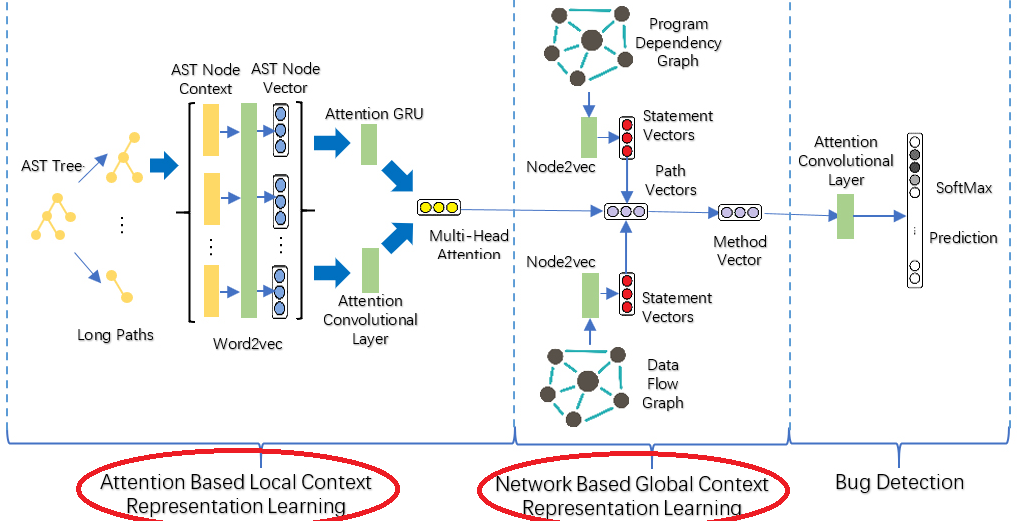
\includegraphics[height = 1.98in]{graphs/Graph_2_trim.png}
	\vspace{-22pt}
	\caption{Using Representation Learning for Bug Detection}
	\label{Fig.2}
%	\vspace{-10pt}
\end{wrapfigure}
(2) \textbf{Network-Based Global Context Representation Learning}.  We
also encode the method's context by building the PDG and the DFG
relevant to the method.
%We call them the \textbf{global context} as they provide the relations
%between the given method and other relevant methods in the project.
We use the Node2Vec~\cite{Grover-2016} to encode the PDG and DFG into
embedded vectors. These two vectors are combined by the space vectors
of all nodes in each path. We use matrix multiplication and convert
results together to get the path representation vector. Then, we can
have a method representation by appending all paths' vectors for each
method.  (3) \textbf{Bug Detection}. With both contexts for a method,
a classifier decides if the method is buggy or not. 

We plan to (1) investigate new CRL via our
framework to integrate program slices/reduction, symbolic traces, code
abstraction and intermediate representations; (2) explore new
embeddings and learning models for different level detection; (3) study new DL models on vectors from CRL to identify bugs.

%Our preliminary results~\cite{oopsla19} showed that with
%representation learning mechanisms (Figure~\ref{Fig.2}), our model
%significantly outperforms the one with the off-the-shelf
%Word2Vec-based CRL.

%\begin{wrapfigure}{r}{0.57\textwidth}
%	\vspace{-10pt}
%	\centering
%	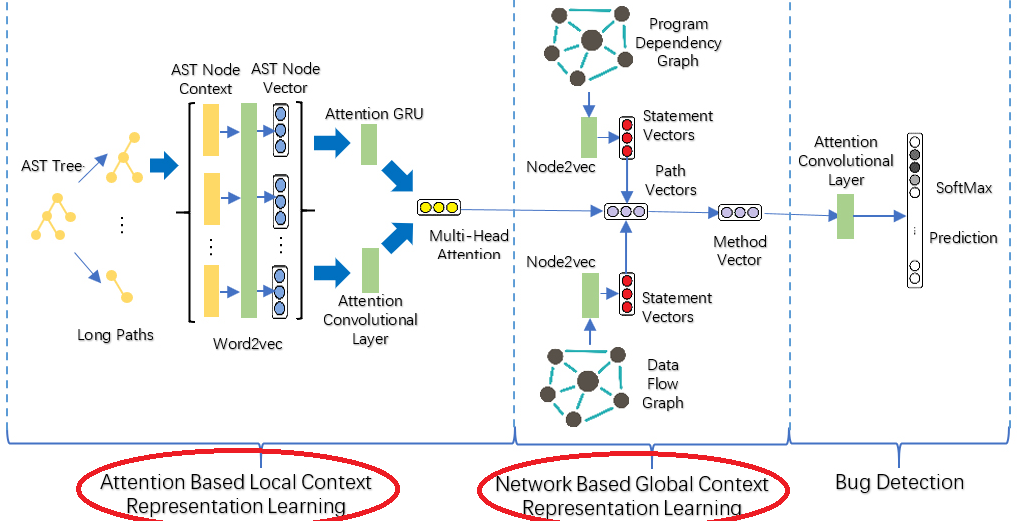
\includegraphics[scale=0.265]{graphs/Graph_2_trim.png}
%	\vspace{-25pt}
%	\caption{Using Representation Learning for Bug Detection}
%	\label{Fig.2}
%	\vspace{-15pt}
%\end{wrapfigure}

%Tien removed
%Table~\ref{allresults} show that (1) \textbf{our initial design
%  outperforms state-of-the-art baselines in detecting bugs},
%relatively improving DeepBugs, Bugram, NAR-miner, and FindBugs by
%69\%, 25\%, 92\%, and 156\% respectively in terms of F-score. (2)
%\textbf{our CRL with local and global contexts is more suitable than
%  existing CRL in bug detection}. It can improve relatively over all
%CLR baselines: DeepSim, DL-similarity, code2vec, Tree-based LSTM, Code
%Vectors,and GGM by 67\%, 38\%, 82\%, 206\%, 101\%, and 16.3\%,
%respectively, in terms of F-score. Importantly, our false positives
%rate is lower than others.
%\begin{wraptable}{r}{0.7\textwidth}
%	\vspace{-15pt}
%	{\footnotesize	
%		\caption{Ours Compared with BD Baselines and Existing CRL on BD. FP: False Positives}
%		\vspace{-10pt}
%		\begin{center}\label{allresults}
%			\renewcommand{\arraystretch}{1}
%			\begin{tabular}{p{1.2cm}<{\centering}|p{0.8cm}<{\centering}|p{0.8cm}<{\centering}|p{0.8cm}<{\centering}|p{1cm}<{\centering}|p{0.8cm}<{\centering}
%					|p{0.8cm}<{\centering}|p{0.8cm}<{\centering}|p{0.8cm}<{\centering}|p{0.8cm}<{\centering}|p{0.8cm}<{\centering}|p{0.8cm}<{\centering}} \cline{2-12}
%				
%				
%				\hline
%				\multirow{2}{*}{Category}& \multicolumn{5}{c|}{Bug detection baselines} & \multicolumn{6}{c}{Existing CRL on bug detection}\\
%				\cline{2-12}
%				& \textbf{Ours} & \textbf{DB} & \textbf{Bram} & \textbf{NARM} & \textbf{FB}   &\textbf{DS} & \textbf{DLS} & \textbf{C2V} & \textbf{TL} & \textbf{CV}&\textbf{GGM}\\
%				\hline
%				Recall  & 0.68 & 0.62 & 0.64 & 0.72 & 0.76   & 0.67 & 0.71 & 0.69 & \textbf{0.82} & 0.70&0.73\\
%				Precision& \textbf{0.39} & 0.25 & 0.32 & 0.11 & 0.08  &  0.19 & 0.24 & 0.17 & 0.09 & 0.15&0.30\\
%				F-score & \textbf{0.50} & 0.36 & 0.43 & 0.19 & 0.14 & 0.30 & 0.36 & 0.27 & 0.16 & 0.25&0.43\\
%				FP Rate & \textbf{0.21} & 0.41 & 0.39 & 0.52 & 0.66 & 0.35 & 0.36 & 0.43 & 0.69 & 0.45&0.28\\
%				\hline
%			\end{tabular}
%			DB=\deepbugs~2018: A deep learning bug detector; Bram=\bugram~2016: A n-gram model based detector;
%			NARM=\narminer~2018: A rule-based static detector mines negative rules on the code;
%			FB=\findbugs~2007: A rule-based static detector encoding +300 bug patterns.
%			DS, DLS, C2V, TL, CV, and GGM are defined in \textbf{Table 2}.
%			
%		\end{center}
%		\vspace{-25pt}
%	}
%\end{wraptable}

%Our initial results confirm that effective code representation learning (CRL) can help improve bug detection.



%Besides the basic CRs, e.g., identifiers/tokens/data and control
%flows/program dependency graph, we plan to investigate code
%representations obtained from more program analysis techniques (static
%and dynamic), such as program slices/reduction, symbolic traces, code
%abstraction, code intermediate representations (IR). Then, we combine
%the basic ones with the representations obtained from more static and
%dynamic program analysis techniques.  (2) Exploring new embeddings and
%learning models to propose new CRL approaches specialized for bug
%detection at different levels (i.e., variables, statements, and
%methods).  (3) Studying and proposing new deep neural networks on code
%vectors generated from CRL to identify bugs.


\subsection{T3 Task 2. Test Code Representation Learning for Regression Testing in CI}

%We use code representation learning to improve the
%selection and prioritization of test cases in Continuous
%Integration (CI)~\cite{duvall2007continuous}.
%
Regression Testing (RT) in Continuous
Integration~\cite{duvall2007continuous} (RT-CI) differs from the
traditional RT because most traditional RT techniques cannot be
applied at the scale of modern CI
practices~\cite{elbaum2014techniques} that require frequent commits to
the shared code base and cause the cost of continuous RT escalate
dramatically~\cite{memon2017taming}.
%
%RT-CI requires to identify and prioritize a subset of test cases that
%can timely and effectively uncover potential regression faults in the
%latest committed changes.
%
%Test selection and prioritization approaches in RT-CI are
%mainly in two directions: heuristics-based approaches
%(e.g.,~\cite{elbaum2014techniques,gligoric2015practical,yu2018study})
%and machine learning based approaches. However, existing approaches,
%e.g.,~\cite{bertolino2020learning,spieker2017reinforcement} still have
%limitations in accuracy and scalability as they lack the learning of
%deep features of test cases and source code and their relations.


%^Both only selection without prioritization or vise versa may be
%unsatisfactory, as time intervals among commits are very short and not
%all selected tests can be run or avoiding running many non-failing or
%irrelevant tests is the goal.
We will design a deep learning approach that leverages code representation
learning to select test cases and then prioritizes them in
each CI cycle.  
(1) \textbf{Test Selection.}  We use a hybrid strategy to select a subset of test cases, considering
static class-level dependencies among test cases and the ones between
changed source code and test cases, newly added test cases, diverse
test cases (e.g., \cite{jiang2009adaptive,henard2016comparing}). 
Static techniques are preferred over dynamic ones that are impractical
in CI due to runtime overhead~\cite{bertolino2020learning}. 
(2) \textbf{Test Prioritization.} Unlike previous approaches
(e.g.,\cite{bertolino2020learning}) modeling source code and test
history using hand-crafted metrics, we use CRL techniques (e.g.,
preferably unsupervised word embedding algorithms such as
Word2Vec~\cite{word2vec}, ELMo~\cite{peters2019knowledge},
FastText~\cite{bojanowski2017enriching}) to learn deep features of the
code under test to vectors, selected test cases, annotations for tests in code, 
similarities between
test cases and changed code, history-based test information (e.g., the
failed tests in the current commit and their similarities with the
changed code, the failed tests per test class in previous commits
before the current one, execution times).  Then, we utilize
learning-to-rank framework or active learning to prioritize test cases. 
In terms of
time complexity, existing approaches still have to generate graphs
(e.g., call/control graphs) for building metrics in a cycle, which can
take a longer time. In our approach, we build a language model
off-line and apply it on the natural sequences (or just tokens or AST)
of code under test into a vector in a cycle, which may not add overhead and even faster.  
Based on our previous experience, CRL can generate deeper and more representative
features than the hand-crafted metrics, leading to better results. 
We will further (1) investigate different
strategies for selection with CRL; (2) explore new fast and efficient
embeddings and learning models to propose new CRL approaches
specialized for RT-CI; (3) study to propose new practical
CRL-based approaches for test prioritization.



%study to propose a new off-line training for costly but potentially useful features and on-line prediction approach. 


%We exclude coverage-test selection and prioritization as they are very costly in CI due to the costs of instrumentation, recording and maintaining coverage data per release, in addition, they provide low accuracy due to the quick cycles and code changes


%different relationships: test cases dependency, dependency between test cases and source code, source code analysis for selecting and prioritizing test cases


\subsection{T3 Task 3. Code Coverage RL, Relation RL, and CRL for Fault Localization}

\begin{wrapfigure}{r}{0.45\textwidth}
	\vspace{-12pt}
	\centering
	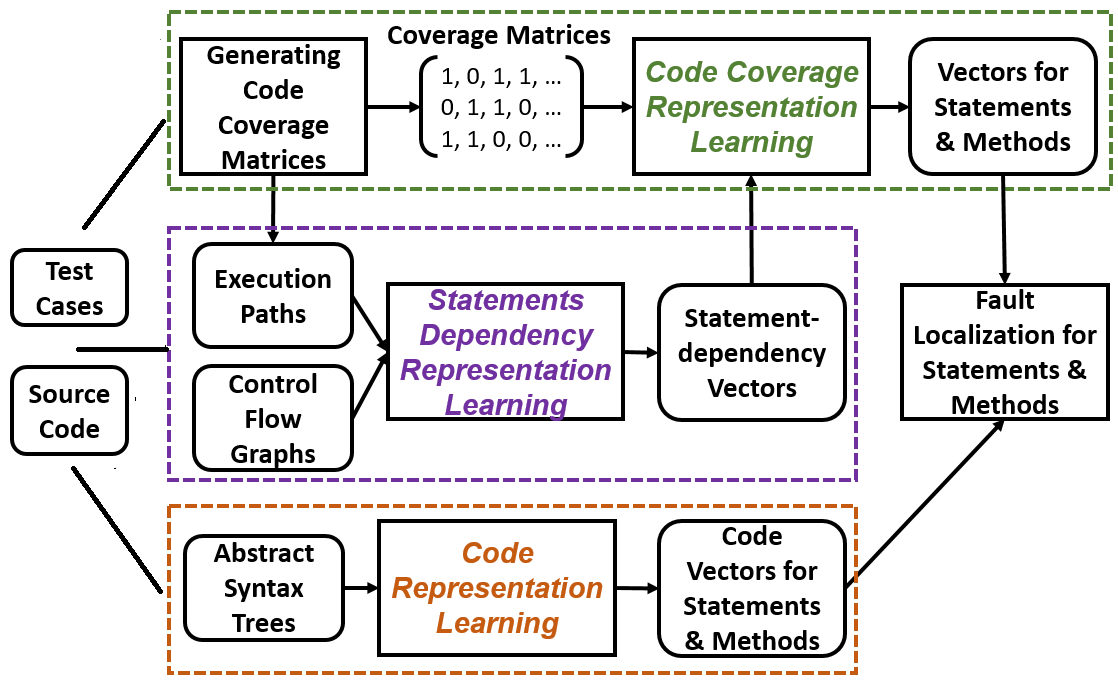
\includegraphics[height=1.8in]{graphs/newOverview}
	\vspace{-20pt}
	\caption{Using Representation Learning in FL.}
	\label{floverview}
	\vspace{-10pt}
\end{wrapfigure}
To experiment with CRL for dynamic information from program
executions, we propose a customized CRL for a fault localization
approach~\cite{icse_fl_21} at the statement and method levels.
%
%We use effective code and test coverage representation learning and
%novel deep neural networks for localizing faults at statement and
%method levels.
Our preliminary design~\cite{icse_fl_21} (Figure~\ref{floverview}) was
to leverage representation learning (RL) in three aspects. (1) {\bf
  code coverage representation learning}: Existing approaches
(spectrum-based, mutation-based, and deep learning-based approaches)
have never used the full details of test coverage, instead, they use
the spectrum and(or) mutation based formulas to summarize test
coverage for all test cases on each statement. We propose to {\em
  treat the FL problem as image processing by learning code coverage
  representations on the full details of the test coverage matrix}.
%Existing approaches (spectrum-based, mutation-based, and deep
%learning-based approaches) have never used the full details of test
%coverage, instead, they use the spectrum and(or) mutation based
%formulas to summarize test coverage for all test cases on each
%statement.
%To enrich test coverage matrices, we extract failing information of a
%test case and link it with specific code statements.  We use -1 for a
%failing test case at a statement exhibiting a crash or incorrect
%value.
%
%Next, while the rows representing statements are arranged according to
%the appearance order in the code, we order the columns, representing
%the test cases, so that the test coverages (i.e., the -1s, 0s, and 1s
%in the test coverage matrix) around the buggy statement would form a
%characteristic ``visual'' feature for a DL model to learn and detect
%it.  We directly perform RL on the improved matrices to learn vectors
%for statements or methods.  \underline{Second}, we integrate the
%dependencies/relations among the statements in the fault localization
%process using data dependency and execution traces.
(2) {\bf Statement dependency representation learning}: we aim to
learn the data/control dependencies among the statements. (3) {\bf
  code representation learning}: we also conduct CRL on sub-trees and
long paths of ASTs to generate vectors for source code. Finally, we
combine all three types of representation learning to represent a
statement or method by a vector representation. We will explore
different DL models for the classification purpose.~Preliminary
work shows that CNN works well for this classification of
a method/statement into buggy or not.

%(1) We prioritize test cases and mine failing information of test
%cases to enrich test coverage matrices and learn the code coverage
%representations; (2) We conduct the CRL on sub-trees and long paths of
%ASTs to generate vectors for source code, and also generate data flow
%graphs and run test cases to collect execution paths of code
%statements to learn the statement dependencies; (3) We combine the
%data flow graph and execution paths with improved matrices (spectrum
%and mutation), then apply a \cnn~on new matrices to learn vectors for
%an improved matrix.  We use another CNN on code vectors, vectors for
%the improved spectrum--based matrices, and vectors for the improved
%mutation-based matrices to perform fault localization (FL) at
%method-level. Our design can also work on statement-level FL by
%replacing the CRL at statement-level.


%\begin{table}[h]
%	\vspace{-15pt}
%	
%	{\footnotesize	
%		\caption{Our Approach Compared with FL Baselines at method-level and statement-level on Defects4J having 395 Bugs in total}
%		\begin{center}
%			\renewcommand{\arraystretch}{1}
%			\begin{tabular}{p{1cm}<{\centering}|p{0.8cm}<{\centering}|p{1cm}<{\centering}p{1cm}<{\centering}p{1cm}<{\centering}p{1.5cm}<{\centering}
%					p{1.2cm}<{\centering}p{1.5cm}<{\centering}|p{1.6cm}<{\centering}p{1.5cm}<{\centering}p{0.8cm}<{\centering}p{1.2cm}<{\centering}|p{0.8cm}<{\centering}} \cline{2-13}				\hline
%				\multirow{2}{*}{}& \multicolumn{7}{c|}{Fault Localization at Statement-Level} & \multicolumn{5}{c}{Fault Localization Method-Level}\\
%				\cline{2-13}
%				& \textbf{Ours} & \textbf{Ochiai} & \textbf{Dstar} & \textbf{MUSE} & \textbf{Metallaxis} &\textbf{RBF-NN} & \textbf{DeepFL-S} &\textbf{MULTRIC} & \textbf{FLUCCS} & \textbf{TraPT} & \textbf{DeepFL}&\textbf{Ours}\\
%				\hline
%				Top-1  & \textbf{74} & 17 & 19 & 26 & 24   & 16 & 36 & 80 & 160  & 156 & 213 &    \textbf{242} \\
%				MFR & \textbf{19.97}& 46.51 & 39.47 & 32.51 & 31.42 & 20.96 & 21.89  & 37.71 & 16.53 & 9.94 & 6.63 & \textbf{6.21}\\
%				\hline
%			\end{tabular}
%			RBF-NN: RBF Neural Network,
%			DeepFL-S: DeepFL with only features from spectrum+Mutation+MLP applicable to statements,
%			Top-1: the number of faults with a least one faulty element (statement or method) within top-1 position,
%			MFR: Mean First Rank of the localization of the first faulty element.
%			All method-level FL are machine learning (incl. deep learning) based.
%			\label{FL_S_M}
%		\end{center}
%		\vspace{-20pt}
%	}
%\end{table}


%Table~\ref{FL_S_M} show that our initial approach outperformed all baselines at both statement and method levels. Compared with the best performing statement-level and method-level baseline: DeepFL-S and DeepFL, we improved them by 115\% and 14\%, respectively. Our key ideas of designing representation learning for code and test coverage can help improve the current state-of-the-art FL research.

%To expand our initial design, we will (1) derive new code representations for FL; (2) Explore new embeddings and learning models to propose new code representation learning (CRL) approaches for FL; (3) Study and proposing new deep neural networks to localize faults.

\subsection{T3 Task 4. Code Transformation Learning for Automated Program Repair}

In this task, we aim to improve DL-based APR approaches via effective
CRLs, particularly {\bf Code Transformation Learning}.
%to improve the current deep-learning (DL) and pattern APR approaches
%using effective CRL and novel deep neural networks.  The DL-based
%approaches, e.g.,~\cite{hata2018learning,lutellier2020coconut}, still
%have limitations in learning bug-fixing code changes and learning
%which context of the surrounding source code that certain bug-fixing
%changes should be made.  These limitations lead to incorrect fixing
%locations or incorrect fixes.
We initially designed a two-tier DL model, \tool~\cite{icse_fl_20}, to
treat APR as code transformation learning from the prior bug fixes and
the surrounding code contexts of the fixes.
%
%For training, {\tool} has 5 key steps: {\bf (1) Pre-Processing.}
%First, {\tool} performs alpha-renaming on the names of variables
%within a method of a project.  Second, , {\tool} uses
%Word2Vec~\cite{Mikolov-2013} to train a vector representation for each
%unique token in a given pair of buggy method ($M_b$) and its fixed
%version ($M_f$).  {\tool} identifies the buggy sub-tree ($T^{sub}_b$)
%within $M_b$, and $T^{sub}_b$'s corresponding changed sub-tree
%($T^{sub}_f$) within $M_f$.  Finally, we used a code summarization
%model~\cite{wan-ase18} to summarize a tree into a vector for a node
%({\em a summarized node}). We obtain one vector for $T^{sub}_f$ and
%another one for $T^{sub}_b$.
{\bf (1) Code Context Learning.} We designed a two-layer learning model
that leans the code transformations for bug fixes and the context of
the code surrounding the fixes. The first one is dedicated for local
\textbf{C}ontext \textbf{L}earning \textbf{L}ayer (CLL).
%
For training at this layer, we replace the changed sub-tree with
a {\em summarized node}, as well as the buggy
sub-tree.  Given pre-processed pairs of methods, we developed a
tree-based encoder-decoder model using tree-based
LSTMs~\cite{tai2015improved} for this local context learning.  We
compute the vector for a method AST with the summarized node in a pair
of methods ($M_b$, $M_f$). The obtained vectors are used as the weights
in the next step. {\bf (2) Code Transformation
	Learning.}  The second layer is dedicated to code
\textbf{T}ransformation \textbf{L}earning \textbf{L}ayer (TLL) for
bug-fixing changes. In TTL, the changed sub-tree before and after the
fix is used for training to learn the bug-fixing code
transformations. Moreover, the context of the transformation computed
as the vector in the context learning layer is used as an additional
input in this~step.
%Specifically, we use the same tree-based encoder-decoder model in the
%first layer, CLL, to encode both structural and token changes.  {\bf
%  (4) Program Analysis Filtering.}  {\tool} derives the possible
%candidates using program analysis filters, including the filter to
%check the existence of variables, methods, and class names, the filter
%to convert the keywords back to the right names, and the filter to
%check the syntax of final result.  {\bf (5) Patch Re-ranking.} We use
%a CNN~\cite{kim2014convolutional} based classification approach to
%re-rank the generated possible patches based on the detailed
%contextual information, which helps better selecting the results.

We also have the following tasks in this thrust: (1) Investigating new
code representations for APR using our code representation learning
(CRL) framework; (2) Exploring new embeddings and learning
models to propose new CRL approaches specialized for APR; and (3)
Studying and even proposing new deep neural network models to auto-fix
multi-statements and multi-location bugs.

%In our initial design, our DLFix is novel in two ways: new CRL and a
%new two-layer tree-based encoder-decoder model.




%\input{benchmark}

%\input{model}
%\input{mudetect}

%\input{solution}


%\input{formal}
\section{Evaluation Plan}
\label{eval}

%Our {\em goals} of the evaluation plan include the studies to answer the questions:

%1) {\bf Intrinsic evaluation.} 

%2) {\bf Extrinsic evaluation.} How well do our proposed tools and methods help developers in improving the learning and usages of APIs in software libraries?

%3) How effectively do the proposed tools and methods help developers
%in real development processes?


\paragraph{\bf (1) Partial-Code Analysis Performance.} We aim
to evaluate how well {\tool} can provide the structural analysis and
semantic analysis for incomplete code fragments.  Assessing the
performance of \tool is not straightforward, mainly due to the lack of
ground-truth for partial code fragments. Thus, we could evaluate it on
programs in Java and C/C++ as follows.  First, we will train {\tool} on
complete code. For testing, we will treat each method individually and
choose a consecutive portion within the method to predict the actual
elements and dependencies, and compare them against the actual ones.
For example, in Thrust 1, if we evaluate the performance of structural
analysis infrastructure, we could compare the recovered/predicted code
structure in terms of ASTs against the actual ASTs of the original
code. For Thrust 2 in dependency analysis, we could treat each method
individually and choose a consecutive portion within the method to
predict the program dependencies, and compare them against the actual
dependencies. We will adopt the standard evaluation metrics, i.e.,
\textit{Accuracy}, \textit{Precision}, \textit{Recall}, and
\textit{F-Score}. $Accuracy = \frac{TN+TP}{TN+FP+TP+FN}$, $Recall =
\frac{TP}{TP+FN}$, $Precision = \frac{TP}{TP+FP}$, and $F{-}Score =
\frac{2*Recall*Precision}{Recall+Precision}$ where TP = True
Positives; FP = False Positives; FN = False Negatives; TN = True
Negatives.

\paragraph{\bf (2) Complete-Code Analysis Performance.}
We aim to compare the performance of {\tool} (AI/ML + PA) against the
traditional PA techniques in building structures and dependencies from
source code. We could collect a set of tools, e.g., to build the
program dependence graphs to obtain the benchmark. Then, we will
compare the results from {\tool} and other tools w.r.t. the
benchmark. We will also measure the time efficiency in building the
infrastructures such as ASTs or PDGs from all the tools under
comparison. We will use the same evaluation metrics as in the
experiments for incomplete code.

\paragraph{\bf (3) Usefulness Evaluation on Downstream Tasks.}

{\em We evaluate how well {\tool} helps in the downstream software
  engineering tasks for partial code}. For example, in bug and
vulnerability detection for code snippets, to evaluate the usefulness
of the PDGs predicted by \tool (say, PDG\textsuperscript{*}), we
will design experiments around the task of vulnerability detection at two
levels of granularity: complete code at the method-level, and partial
code at the snippet-level. For the method-level VD task, we leverage
any ML-based vulnerability detection tool, e.g.,
VulCNN~\cite{wu2022vulcnn}, an image-inspired DL-based VD model which
utilizes PDGs to predict whether a given method has vulnerabilities or
not. Here, we aim to estimate how well PDG\textsuperscript{*}s
predicted for the methods in the dataset approximate the performance
of the actual PDGs retrieved from a program-analysis tool. We could
use the same methodology for evaluating the usefulness of {\tool} in
other types of software engineering tasks.



%{\em in bug detection (BD), fault localization (FL), Regression
%  Testing in Continuous Integration (RT-CI) and automated program
%  repair (APR) approaches are in comparison with the state-of-the-art
%  approaches?}  First, we use the large-scale cross-language datasets
%with bug fixes.  To detect bugs, we will train our BD and FL
%approaches on buggy code with known buggy locations and non-buggy
%code. For APR, we train APR approaches on buggy code with its fixed
%versions to automatically learn fix patterns. Second, for evaluation,
%we follow prior research for BD, FL, and APR. \underline{In DB}, we
%will measure the precision, recall, F-measure, and the number of true
%bugs detected in Top-N (e.g., N=50). \underline{In FL}, we use the
%following: \textit{Recall at Top-N}, the number of faults with at
%least one faulty element located within the first N positions.
%\textit{Mean Average Rank (MAR)}: For precise localization of all
%faulty elements of each fault, we compute the average ranking of all
%the faulty elements for each fault.  \textit{Mean First Rank (MFR)}:
%For each project, we compute the mean of the first faulty element's
%rank for each fault.  \underline{In RT-CI}, we calculate APFD (Average
%Percentage of Faults Detected), Normalized APFD
%(NAPFD)~\cite{qu2007combinatorial} and Normalized Rank Percentile
%Average (NRPA)~\cite{bertolino2020learning}. Rank Percentile Average
%(RPA) was proposed to adapt the Average Fault Percentile to the
%prioritization problem for computing how much a predicted ranking is
%close to the actual ranking.  \underline{In APR}, we calculate the
%number of bugs automatically fixed and the ratio of correctly fixed
%bugs to the number of plausible patches when comparing with
%traditional APR approaches. Compared with DL ARP, we use: \textit{Top
%  K is the number of times that a correct patch is in the ranked list
%  of top K candidates, e.g., K=1,3,5}.

%\paragraph{{\bf (2) Comparative Study on Code Representation Learning (CLR) for BD, FL, RT-CI and APR.}}
%{\em Research question: How effective are our CRL for BD, FL, Testing and APR, and how well are they in comparison with the state-of-the-art approaches?} 
%We will perform controlled experiments to evaluate the effectiveness of our CRL in BD, FL, RT and APR, especially ablation studies on different factors in CRL. In addition, we will continue to compare our CRL with other existing CRL on other software engineering and program analysis topics. We use the same evaluation metrics as the ones in (1) for BD, FL, and APR.

%To evaluate our evaluation framework for CRL, we propose the following
%procedure. First, we will choose a well-known DL-based model for each
%application, BD, FL, RT-CI, and APR. For each of those DL-based
%models, we varied the CRL model using our design framework in Thrust
%1. We measure the quality of each CRL model and measure the
%performance of the DL-based model for each application. We will use
%statistical test to evaluate whether the high accuracy of CRL model
%leads to high performance of the same downstream model used in the
%application under study.

%\subsection{Evaluation on usefulness of the approaches in helping developers in learning API usages}

%We will perform controlled experiments to evaluate our methods and tools with developers in the loop using the actual system. We will
%gather developers and provide them various programming tasks, and
%compare the efficiency of their work with our methods/tools to the
%baseline approaches, e.g., with the Web-based code search or other
%code synthesis approaches.

%We will measure the efficiency of the work using different methods
%based on the following evaluation metrics. First, we measure
%efficiency. This could be measured by the time for developers to
%perform the tasks or the number tasks completed by developers in a
%period of time. Second, we measure coding effort: how much effort that
%developers must do to complete the API usages given the API code from
%the methods. Third, we will measure semantic correctness, either by
%the number of passing test cases or by human judgements. Finally, we
%will perform surveys on the quality of the synthesized API usage code
%to get the feedback for future improvement in the next step.

\paragraph{\bf (4) Evaluation on proposed tools and methods in helping developers in real-world development.}

We will perform a set of user studies on the usefulness of our
proposed tools in the wild by releasing our
tools in the actual real-world development. 
%We will analyze all the aspects as in the previous studies and the total uptake of the tools.  
We will record feedback to improve our tools.
%PI Wang will connect with the Industry through our \textit{The New Jersey Innovation Institute} (NJII)~\cite{njii}, an NJIT corporation focusing on helping pri%vate enterprise.
UT-Dallas has a strong tie with companies like AT\&T, Facebook, and
Bloomberg. PI Nguyen will work with his existing collaborators in
Microsoft, IBM, ABB research to perform user studies on the groups of
developers in certain tasks to evaluate the usefulness of our proposed
tools.

%\section{Education and Dissemination Plan - Curriculum Development Activities}
\section{Dissemination and Educational Plan}
\label{edu}

\paragraph{Engaging Students into Research}

This project will create opportunities for students at UT-Dallas to
participate into cutting-edge research: PI Nguyen has currently supported
four female students (2 PhD students and 2 undergraduates), with a total
of four PhD students, two M.Sc. students, and four undergraduates.

%has worked with 6 undergraduate students (i.e., two are female
%students) and two master students (i.e., independent
%study). Additionally, PI Wang is actively doing research with a group
%of two undergraduate students (Vrushali Koli (female) from NJIT and
%Delmond Wyllis from Rowan Univ. in NJ) and \underline{six high-school
%students} in the NJ Governor's STEM Scholars Program.  PI Wang
%supervise 4 Ph.D students (one female) and 1 master student.


%(2) {\em UTD's Collegium Honors Program}:
%{\em ISU's Freshman Honor program}: 
%PI Nguyen has been engaging two freshman honor students into his
%research program since he joined UTD in 2016. 
%REU supplements will be requested to support this undergraduate research; 
%
%(3) {\em HackersUTD}: This Fall, UT Dallas Computer Science department
%welcomed 2,876 students, including 466 CS/software engineering
%freshmen, with activities and events as a way to welcome and
%familiarize students with the UT Dallas CS. We will engage members of
%this organization; 
%(3) UT Dallas works with North Texas high school
%seniors to host IT empowerment for their camps. To generate interests
%in computing studies from {\em high-school} students in Dallas area,
%we will involve them in design projects that target the use of
%software in teaching {\em K-12} subjects; 
%(2) {\em UTD's Women Who
%Compute}: The PI Nguyen has actively used this program to generate interests
%in SE research from women students. From the past, PI Nguyen has
%mentored 3 women students; 
%(Dong Fei, Kristina Gervais, Taylor Schreck); 
%(3) {\em Involving Under-represented Minorities}: We
%will attract minority students funded by GEM fellowships, involve
%high-school teachers via Alliances for Graduate Education and the
%Professoriate.
%and UT Dallas Programs for Minors: we will work
%with this program to recruit more student in minority.

%This project will also create opportunities for students at UT-Dallas:
PI Nguyen has extensive experience in engaging students in
outreach programs: (1) {\em UTD's Collegium Honors Program}: He
has been engaging several freshman honor students into his research
program since 2005. (2) {\em HackersUTD}: In Fall'19, UT Dallas CS
welcomed 2,876 students, including 466 freshmen, with activities and
events as a way to familiarize students with CS/SE. We will use the
results of this project in this program.
%
(3) UT Dallas works with {\em North Texas high school seniors to host
IT empowerment} for their camps. To generate interests in computing
studies from {\em high-school} students in Dallas area, PI Nguyen has
been involving them in design projects that target the use of software
in teaching {\em K-12} subjects; (4) {\em UTD's Women Who Compute}: he
has actively used this program to generate interests in SE research
from women students. PI Nguyen has mentored several {\em female
undergraduate students} (Weining Gao, Kristina Gervais, Taylor
Schreck, etc.); (4) {\em Involving Under-represented Minorities}: We
will attract minority students funded by GEM fellowships, involve
high-school teachers via Alliances for Graduate Education and the
Professoriate; and (5) {\em UT Dallas Programs for Minors}: we will
work with this program to recruit more student in minority.


\paragraph{Dissemination of Research and Teaching Materials}

Beside publications at professional \emph{conferences, journals} and
public Web sites, we will use the available resources at UT-Dallas
through various forums for dissemination.
%
%PI Wang is a member of DIMACS~\cite{dimacs}, the Center for Discrete
%Mathematics and Theoretical Computer Science as an NSF-funded Science
%and Technology Center (STC) and a New Jersey Commission on Science and
%Technology Advanced Technology Center. DIMACS has over 350 members
%across the U.S. PI Wang will continue to advocate our research through
%DIMACS events, research and academic programs.  PI Wang will use
%the \textit{annual NJIT Research Showcase and President Forum} to show
%our accomplishments to all NJIT people.
PI Nguyen will continue to use the following resources: (1) TExAs
Software Engineering Research (TEASER) Doctoral Symposium: where SE
researchers from the DFW Metroplex (and beyond) meet to discuss and
work on SE topics.  The mission of TEASER is to provide a supportive
space in which PhD students can present and receive feedback on their
research work, while at the same time giving both researchers and
students a venue to get to know one another and network productively.
(2) American Society for Engineering Education: PI Nguyen, with his
prior NSF-funded TUES project, has disseminated educational results
via this channel.
%He will continue to disseminate educational outcomes via this
%educational society.
(3) Leadership through Engineering Academic Diversity (LEAD): PI
Nguyen have served as mentors for this program which aims to enrich
educational experience of {\em minority engineering students}.

\paragraph{Research Community Building.}

PI Nguyen has successfully organized the 1st {\bf International
Workshop on Representation Learning for Software Engineering and
Programming Languages (RL+SE\&PL 2020)}~\cite{rlsepl}, associated with
ESEC/FSE'20. The workshop had 104 paid registers and featured one
keynote speaker (Dr. Miltos Allamanis, well-known CRL scientist at
Microsoft Research) and six technical presentations. RL+SE\&PL'20 has
sparked constructive and inspiring discussions. With its success, we
are building a diverse and active community. We plan to build on the
success of the first edition to continue this series to disseminate
ideas to a wider community, and to build a larger community bridging
SE and ML.


\noindent {\bf Undergraduate and Graduate Software Engineering (SE) Education.} 
%PI Wang teaches fundamental and core SE courses NJIT: Building Web Applications (IS218) and System Design (IS390).
PI Nguyen is one of the key SE faculty members in SE at UT Dallas. 
%
He is one of the faculty who has initiated the
Undergraduate SE Program when he was at Iowa State University.
%He has
%successfully introduced several courses including Software
%Architecture and Design (CprE339) and Software Project Management
%(CprE329). 
Taking advantage of this project, PI Nguyen will introduce a deep
learning component and a new course in NLP+SE.
%The key teaching philosophy in this course is the combination of theory and practice.
%in which students will be introduced different principles and theories in the application of NLP in SE artifacts. 
%The tentative modules include 1) basic principles, processes, and paradigms in NLP, 2) programming languages versus natural languages, 3) API usages and reuse, 4) Statisical models used in SE applications, 5) machine translation and code migration, 6) language models for source code, 7) applications of machine translation in SE, 8) word embeddings and SE applications, 9) deep learning and SE applications, etc.
%\noindent {\em Graduate SE Education} 
PI Nguyen will teach a newly developed course, 
Selected Topics on AI in SE and PL,
including relevant topics to this proposal, e.g, 
AI in bug detection, fault localization, automated repair. 
%The PI Nguyen works
%with other UTD faculty to develop a series of six to seven SE graduate
%courses that will be offered at least every semester. This year, the
PI Nguyen introduced a new graduate level course on ``AI/ML for
Code''. The PI will introduce a new graduate course on the topic of
NLP+SE.
%Tools developed by this research will be used in class projects. 
The course will focus on SE advanced methods that
aim to help advance SE with AI/ML. 
The tentative topics include 1) program analysis, 2) code
analysis with AI/ML, 3) cross-language analysis between texts and code,
4) AI/ML for code, etc.
%4) code and text retrieval in SE applications, 
%3) NLP techniques and
%type inference, 4) NLP and de-ofuscation, 5) bug-fixing and
%machine learning.




%\input{ccf20-plan}
%\input{priorsupport}
\section{PI's Prior Relevant NSF Supports and Qualifications for this Project}
\label{prior}

%PI Wang has no prior relevant NSF supports.
%His relevant work on improving software maintenance, quality and reliability has been published in
%OOPSLA~\cite{yioopsla19}, ASE~\cite{son-2019-ase}, EMSE~\cite{noei2019towards,wang2016improving}, ICWS~\cite{venkatesh2016client}, ICSOC~\cite{wang2014developers}, and MSR~\cite{wang2013improving,wang2019extracting}.
%two ICSE submissions, and one PLDI submission.
PI Nguyen. CCF-1723215, \$260,709, 07/01/16-30/06/21, ``Collaborative
Research: Exploiting the Naturalness of Software''.
%
\noindent {\bf Intellectual Merit.} The work has the following
thrusts: (1) investigating NLP techniques for SE
applications, and (2) Developing a statistical machine translation
model for language migration.
%Investigating the integration of semantic information
%including data types, semantic roles, etc., into a language model, (2)
%Developing an accurate code-completion tool using statistical semantic
%language model, and (3) Developing a statistical machine translation
%model for language migration.
%
\noindent {\bf Broader Impact.}
%We developed practical software engineering tools, using statistical
%NL techniques for (a) code suggestion, completion, and correction
%tools, (b) assisting tools for programmers, (c) summarization, (d)
%retrieval, and (e) porting tools.
%The project has several publications at top-tier SE
%conferences, e.g., ICSE, FSE, ASE, TSE.
%including ICSE
%papers~\cite{icse05,icse07,icse09,icse10,icse11}, FSE
%papers~\cite{fse06,fse09,fse11}, ASE
%papers~\cite{ase06,ase08,ase08-2,ase09,ase10,ase11-phpsync,ase11-bugscout,ase11-idiff},
%OOPSLA papers~\cite{oopsla04,oopsla06,oopsla10}, and TSE
%papers~\cite{tse08,tse11}.
%
He has been awarded {\bf 4 ACM SIGSOFT Distinguished Paper Awards, one
  Best Paper Award, and one best ICSE Formal Research Demonstration
  Award} at the top-tier SE conferences including ICSE, FSE, and ASE,
one {\bf IEEE TCSE Distinguished Paper Award}. He has served on
Program Committees and Program Boards of ICSE, FSE, ASE, OOPSLA,
ECOOP. PI Nguyen was a Program Co-Chair of ASE'17. Since 2005, PI
Nguyen published at the top-tier Software Engineering conferences: 25
ICSE full papers, 15 ESEC/FSE full papers, 14 ASE full papers, 3
OOPSLA full papers.
%From Google Scholar, PI Nguyen's H-index
%is 49, Citations: 9,431, Citations in past 5-years: 5,879.
From CSRankings, he is ranked at the 3rd place among all US SE researchers in the past 10 years.

%making software development more accessible, enjoyable and productive;
%and therefore will broadly enhance the value that software
%professionals deliver to business and society.

%Dr. Nguyen is currently the PI of the NSF-funded project, ``
%Collaborative Research: Exploiting the Naturalness of Software'', that
%will end August 2018. The work has three thrusts of research.  (1)
%Investigating the integration of semantic information including data
%types, semantic roles, etc., into a language model, (2) Developing an
%accurate code-completion tool using statistical semantic language
%model, and (3) Developing a statistical machine translation model for
%language migration. So far, the majority of the tasks have been
%%completed except empirical evaluation in a real-word setting is
%needed.



%Several papers on our results were published through ICSE
%2010~\cite{icse10}, ASE 2010~\cite{ase10}, OOPSLA
%2010~\cite{oopsla10}, ICSM 2010~\cite{icsm10}, ICSE
%2011~\cite{icse11,nier11-1,nier11-2}, FSE 2011~\cite{fse11}, ASE
%2011~\cite{ase11-phpsync,ase11-bugscout,ase11-idiff}, and an IEEE TSE
%journal article~\cite{tse11}.

%Our next phase will be involved more with the tasks (2) and (3).

%Dr. Nguyen is currently an PI on a NSF-funded project: \#CCF-1018600,
%``Find and Fix Similar Software Bugs'', 08/15/2010 through
%07/31/2013. In this project, an empirical study will be conducted to
%collect, analyze, and understand the nature and characteristics of
%recurring and similar bugs within one and across multiple
%systems. This project is expected to advance software engineering
%knowledge on the theoretical foundation, concepts, practical
%techniques, and automated tools to (1) capture the characteristics and
%measure the similarity of code units involved in prior known fixed
%bugs, (2) identify the locations of potential buggy units and derive
%the guidelines to fix them by matching them to the relevant peer code
%units of the known bugs, and (3) support the similar bug detection and
%fixing process. Teaching modules and validation efforts in this
%project will involve students and professionals, promoting teaching
%and training software quality assurance.

%Dr. Nguyen is an expert in software building, software configuration
%management (SCM), and software refactoring. His research work on SCM
%has been published at various prestigious software engineering
%journals and conferences including clone-aware configuration
%management and operation-based version control (TSE'11~\cite{tse11},
%FASE'10~\cite{fase10}, ASE'09~\cite{ase09}), software
%refactoring-aware SCM and software merging (TSE'08 \cite{tse08},
%ICSE'07~\cite{icse07}, FSE'06~\cite{fse06}, OOPSLA'06
%demo~\cite{oopsla06}), object-oriented configuration management
%(ICSE'07~\cite{icse07}, WWW'06~\cite{www06}, ICSE'05~\cite{icse05},
%ICSM'05~\cite{icsm05}).

%His other software maintenance works include clone-related bug
%detection (TSE'11 \cite{tse11}), bug localization
%(ASE'11~\cite{ase11-phpsync}), bug localization from bug reports
%(ASE'11~\cite{ase11-bugscout}), recurring bug detection
%(ICSE'10~\cite{icse10}), API misuse detection
%(OOPSLA'10~\cite{oopsla10}, FSE'09~\cite{fse09}), recurring
%vulnerabilities detection (ASE'10~\cite{ase10}), etc.




%Since 2005, his work has been resulting several publications at
%top-tier SE conferences including 5 ICSE
%papers~\cite{icse05,icse07,icse09,icse10,icse11}, 3 FSE
%papers~\cite{fse06,fse09,fse11}, 8 ASE
%papers~\cite{ase06,ase08,ase08-2,ase09,ase10,ase11-phpsync,ase11-bugscout,ase11-idiff},
%2 WWW papers~\cite{www04,www06}, 3 OOPSLA
%papers~\cite{oopsla04,oopsla06,oopsla10}, and 2 FASE
%papers~\cite{fase09,fase10}, 2 TSE papers~\cite{tse08,tse11}.


\newpage
\setcounter{page}{1}
\pagenumbering{roman}

\bibliographystyle{IEEEtran}
%\nobibliography{oopsla19,icse20,FL,ref,autofixTools}
\bibliography{references,oopsla19,icse20,FL,ref,autofixTools,testPri,embeddingEva,reference,icse21IntVD,icse18}

%\bibliography{oopsla19, icseAutoFix20,bibliography,icse18,t2api17,ccf18,refs,securesync,tc10,tien,ccf09,ase10,ccf12,anomalies,completion,groums,usagemining,pattern,urls,other}

\end{document}
